%%%%%%%%%%%%%%%%%%%%% author.tex %%%%%%%%%%%%%%%%%%%%%%%%%%%%%%%%%%%
%
%\documentclass[graybox]{svmult}
%
%\usepackage{mathptmx}       % selects Times Roman as basic font
%\usepackage{helvet}         % selects Helvetica as sans-serif font
%\usepackage{courier}        % selects Courier as typewriter font
%\usepackage{type1cm}        % activate if the above 3 fonts are
                            %% not available on your system
%%
%\usepackage{makeidx}         % allows index generation
%\usepackage{graphicx}        % standard LaTeX graphics tool
                             %% when including figure files
%\usepackage{multicol}        % used for the two-column index
%\usepackage[bottom]{footmisc}
%\usepackage{amsmath}
%\usepackage{multirow}
%\newcommand{\extr}{extr}
%
%\makeindex             % used for the subject index
                       %% please use the style svind.ist with
                       %% your makeindex program
%
%%%%%%%%%%%%%%%%%%%%%%%%%%%%%%%%%%%%%%%%%%%%%%%%%%%%%%%%%%%%%%%%%%%%%%%%%%%%%%%%%%%%%%%%%%
%
%\begin{document}

\title{Sequential and parallel algorithms for multidimensional multiextremal optimization based on the nested  scheme of dimensionality reduction}
\titlerunning{Nested  scheme of dimensionality reduction}
% Use \titlerunning{Short Title} for an abbreviated version of
% your contribution title if the original one is too long
\author{Vladimir A.Grishagin and Ruslan A.Israfilov}
% Use \authorrunning{Short Title} for an abbreviated version of
% your contribution title if the original one is too long
\institute{Vladimir A.Grishagin \at N.I.Lobachevsky State University, Gagarin Avenue 23, 603950 Nizhni Novgorod, Russia   \email{vagris@unn.ru}
\and Ruslan A.Israfilov \at N.I.Lobachevsky State University, Gagarin Avenue 23, 603950 Nizhni Novgorod, Russia 
\email{ruslan@israfilov.com}}
%
\maketitle


\abstract{The dimensionality reduction schemes occupy an important place among the complexity reduction approaches in the multiextremal optimization problems. In the present chapter, one of such schemes, namely, so called nested optimization scheme is considered. This scheme allows one to replace solving a multidimensional problem by solving a family of one-dimensional subproblems nested recursively. Along with a general reduction scheme, its implementation in combination with various global search algorithms is considered. The nested scheme has a considerable potential of parallelization since various one-dimensional parallel optimization algorithms, in particular, the characteristical ones can be applied for solving the internal one-dimensional subproblems. The asynchronism of the parallel computations originating from the recursive nesting of the subproblems is an integral part of the scheme to be considered.}

\section{General nested optimization scheme}
\label{sec:5_1}
Let us consider a nonlinear programming problem in the form 
\begin{equation}
\label{eq:5_1}
\varphi(y)\rightarrow min,y\in Q\subseteq R^N,
\end{equation}
\begin{equation}
\label{eq:5_2}
Q=\{y\in D:g_j(y)\leq 0,\:1\leq j\leq m\},
\end{equation}
\begin{equation}
\label{eq:5_3}
D=\{y\in R^N:a_i\leq y\leq b_i,\:1\leq i\leq N\}.
\end{equation}

Assume that all constraint functions $g_j(y),\:1\leq j\leq m$,  are continuous and the domain $D$  is  bounded that provides the compactness of the feasible domain $Q$. 

Let us introduce a continuous function $G(y)$  defined in the domain $D$  such that
\begin{equation}
\label{eq:5_4}
  \begin{cases}
    G(y)\leq 0, & y\in Q, \\
    G(y)>0, & y\notin Q.
  \end{cases}
\end{equation}

For example, the following functions can be taken as $G(y)$ :
\begin{equation}
\label{eq:5_5}
G(y)=\max\{g_1{y},\;g_2(y),\:\ldots\:,g_m(y)\}
\end{equation}
or
\begin{equation}
\label{eq:5_6}
G(y)=\max\{0;\:g_1{y},\;g_2(y),\:\ldots\:,g_m(y)\}.
\end{equation}
The latter function equals to zero at all points of the domain $Q$.

The following notations
\begin{equation}
\label{eq:5_7}
u_i=(y_1,\ldots,\:y_i),\;v_i=(y_{i+1},\ldots,y_N),
\end{equation}
allow one to write down the vector $y$ as a pair $y=(u_i,\;v_i)$  for $1\leq i\leq N$. Assume that $y=v_0$  if $i=0$  and $y=u_n$  for $i=N$.

Let us introduce  \textit{sections} of the domain $Q$ as
\begin{equation}
\label{eq:5_8}
S_1=Q,\ S_{i+1}(u_i)=\{v_i\in R^{N-i}:(u_i,v_i)\in Q\},\:1\leq i\leq N-1,
\end{equation}
and \textit{projections}
\begin{equation}
\label{eq:5_9}
\Pi_{i+1}(u_i)=\{y_{i+1}\in R^1:\exists (u_{i+1},v_{i+1})\in S_{i+1}(u_i)\},\:1\leq i\leq N-1,
\end{equation}
of the sections $S_{i+1}(u_i)$ onto the axis $y_{i+1}$.

Let us define recursively a family of functions
\begin{equation}
\label{eq:5_10}
  \begin{cases}
    G^N(y)\equiv G(y), \\
    G^i(u_i)=\min\{G^{i+1}(u_i,y_{i+1}:y_{i+1}\in [a_{i+1},b_{i+1}]\},\;1\leq i\leq N-1,
  \end{cases}
\end{equation}
over corresponding projections 
\begin{equation}
\label{eq:5_11}
D_i=\{u_i\in R^i:y_j\in[a_j,b_j],\:1\leq j\leq i\}
\end{equation}
of the domain $D$  from (\ref{eq:5_3}) onto the coordinate axes $y_1,\ldots,y_i$. Moreover, by definition, $D_N=D$.

Because of the continuity of the function $G^N(y)\equiv G(y)$ and of the compactness of the domain $D$ the function  $G^{N-1}(u_{N-1})$ exists and is continuous in  $D_{N-1}$. This fact causes the existence and the continuity of the function  $G^{N-2}(u_{N-2})$ in  $D_{N-2}$ and further determines the existence and the continuity of all functions from family (\ref{eq:5_10}) in corresponding domains (\ref{eq:5_11}). 

The following lemma takes place.
\begin{lemma} 
\label{lem:5_1}
\begin{equation}
\label{eq:5_12}
G^i(u_i)=\min\{G(u_i,v_i):y_j\in [a_j,b_j],\:i+1\leq j\leq N\}.
\end{equation}
\end{lemma}
\begin{proof}
As a consequence of (\ref{eq:5_10}) the assertion (\ref{eq:5_12}) is equivalent to
\begin{equation}
\label{eq:5_13}
\min_{y_{i+1}\in [a_{i+1},b_{i+1}]}\ldots \min_{y_N\in [a_N,b_N]}G(u_i,v_i)=\min\{G(u_i,v_i):y_j\in [a_j,b_j],i+1\leq j\leq N\}.
\end{equation}

Because of the continuity of $G(y)$, for any $u_i\in D_i$ there exists $\bar{v}_i=(\bar{y}_{i+1},\ldots,\bar{y}_N)$ such that $\bar{y}_j\in [a_j,b_j],\:i+1\leq j\leq N,$ and
\begin{displaymath}
\min_{y_{i+1}\in [a_{i+1},b_{i+1}]}\ldots \min_{y_N\in [a_N,b_N]}G(u_i,v_i)=G(u_i,\bar{v}_i)
\end{displaymath}
from where it follows that the left-hand side of the equality  (\ref{eq:5_13}) is greater or equal to the right-hand side. 

Now the subject of our interest is the reverse inequality. Because of the continuity of $G(y)$ and of the compactness of the domain $D$  there exists a vector $v_i^*=(y_{i+1}^*,\ldots ,y_N^*)$  such that 
\begin{displaymath}
G(u_i,v_i^*)=\min\{G(u_i,v_i):y_j\in [a_j,b_j],\:i+1\leq j\leq N\}.
\end{displaymath}

According to (\ref{eq:5_10}), we have
\begin{displaymath}
G^{N-1}(u_i,y_{i+1}^*,\ldots ,y_{N-1}^*)=\min\{G(u_i,y_{i+1}^*,\ldots,y_{N-1}^*,y_N):y_N\in [a_N,b_N]\}\leq G(u_i,v_i^*),
\end{displaymath}
\begin{displaymath}
G^{N-2}(u_i,y_{i+1}^*,\ldots ,y_{N-2}^*)=\min\{G^{N-1}(u_i,y_{i+1}^*,\ldots,y_{N-2}^*,y_{N-1}):y_{N-1}\in [a_{N-1},b_{N-1}]\}\leq 
\end{displaymath}
\begin{displaymath}
\leq G^{N-1}(u_i,y_{i+1}^*,\ldots,y_{N-2}^*,y_{N-1}^*)\leq G(u_i,v_i^*),
\end{displaymath}
$\ldots$
\begin{displaymath}
G^i(u_i)=\min\{G^{i+1}(u_i,y_{i+1}):y_{i+1}\in [a_{i+1},b_{i+1}]\}\leq G^{i+1}(u_i,y_{i+1}^*)\leq G(u_i,v_i^*).
\end{displaymath}
This chain of inequalities finalizes the proof.
\end{proof}

Let us introduce the projections 
\begin{equation}
\label{eq:5_14}
Q_i=\{u_i\in R^i:\exists (u_i,v_i)\in Q\},\:1\leq i\leq N,
\end{equation}
of the domain $Q$ onto the coordinate axes $y_1,\ldots,y_i$.
\begin{lemma} 
\label{lem:5_2}
Projection (\ref{eq:5_14}) can be presented in the equivalent form 
\begin{equation}
\label{eq:5_15}
Q_i=\{u_i\in R^i:G^i(u_i)\leq 0\}.
\end{equation}
\end{lemma}
\begin{proof}
Let  (\ref{eq:5_14}) be fulfilled, i.e., for some $u_i$  there exists $v_i^*$  such that $(u_i,v_i^*)\in Q$. Then, $G(u_i,v_i^*)\leq 0$ , i.e., as a consequence of Lemma \ref{lem:5_1},
\begin{displaymath}
G^i(u_i)=\min\{G(u_i,v_i):y_j\in[a_j,b_j],\:i+1\leq j\leq N\}\leq G(u_i,v_i^*)\leq 0,
\end{displaymath}
and (\ref{eq:5_15}) is true.

Now assume that $G^i(u_i)\leq 0$  for some $u_i\in Q_i$. However, according to Lemma \ref{lem:5_1}, a vector $v_i^*$  exists such that $G^i(u_i)=G(u_i,v_i^*)\leq 0$ , i.e., $(u_i,v_i^*)\in Q$.

Lemma has been proved.
\end{proof}
\begin{lemma} 
\label{lem:5_3}
The definition of the projection (\ref{eq:5_9}) is equivalent to the form 
\begin{equation}
\label{eq:5_16}
\Pi_{i+1}(u_i)=\{y_{i+1}\in [a_{i+1},b_{i+1}]:G^{i+1}(u_i,y_{i+1})\leq 0\}.
\end{equation}
\end{lemma}
\begin{proof}
First of all, note that because of $Q\subseteq D$, for all $y\in Q$ the double inequalities $a_j\leq y_j\leq b_j$,  , hold necessarily. Let $y_{i+1}$  be such that $G^{i+1}(u_i,y_{i+1})\leq 0$ . Then there exists $v_{i+1}^*$  such that $G(u_i,y_{i+1},v_{i+1}^*)=G^{i+1}(u_i,y_{i+1})\leq 0$, i.e., $(y_{i+1}, v_{i+1}^*)\in S_{i+1}(u_i)$. Consequently, $y_{i+1}$  belongs to the projection $\Pi_{i+1}(u_i)$  in the sense of the definition (\ref{eq:5_9}).

Next, for any $y_{i+1}$  satisfying (\ref{eq:5_9}) there exists $v_{i+1}^*$  such that $(y_{i+1},v_{i+1}^*)\in S_{i+1}(u_i)$. Then, the vector $(u_i,y_{i+1},v_{i+1}^*)\in Q$, i.e., $G^{i+1}(u_i,y_{i+1})\leq G(u_i,y_{i+1},v_{i+1}^*)\leq 0$.

The equivalence of (\ref{eq:5_9}) and (\ref{eq:5_16})  has been proved.
\end{proof}
Now consider  a continuous function $\varphi(y)$. Setting $\varphi^N(y)\equiv \varphi(y)$ by definition, let us construct a family of functions 
\begin{equation}
\label{eq:5_17}
\varphi^i(u_i)=\min\{\varphi^{i+1}(u_i,y_{i+1}):y_{i+1}\in \Pi_{i+1}(u_i)\},\:1\leq i\leq N-1,
\end{equation}
defined over the corresponding projections $Q_i$  from (\ref{eq:5_14}). Then, according to \cite{5_CarrHowe} and \cite{5_StrSergMon2000} the basic relation of the nested optimization scheme 
\begin{equation}
\label{eq:5_18}
\min_{y\in Q}\varphi(y)=\min_{y_1\in \Pi_1}\min_{y_2\in \Pi_2(u_1)}\ldots\min_{y_N\in \Pi_N(u_{N-1})}\varphi(y).
\end{equation}
takes place. 

As it follows from (\ref{eq:5_18}), in order to solve the problem (\ref{eq:5_1})--(\ref{eq:5_3}) it is sufficient to solve the one-dimensional problem 
\begin{equation}
\label{eq:5_19}
\varphi^1(y_1)\rightarrow \min,\:y_1\in \Pi_1\subseteq R^1,
\end{equation}
\begin{displaymath}
\Pi_1=\{y_1\in [a_1,b_1]:G^1(y_1)\leq 0\}.
\end{displaymath}

According to (\ref{eq:5_17}), each calculation of the function $\varphi^1(y_1)$  at some fixed point $y_1\in\Pi_1$   requires solving  the one-dimensional problem 
\begin{displaymath}
\varphi^2(y_1,y_2)\rightarrow \min,\:y_2\in \Pi_2(y_1)\subseteq R^1,
\end{displaymath}
\begin{displaymath}
\Pi_2(y_1)=\{y_2\in [a_2,b_2]:G^2(y_1,y_2)\leq 0\}.
\end{displaymath}
This problem is a one-dimensional minimization problem with respect to $y_2$  since $y_1$  is fixed.

In turn, each calculation of the function $\varphi^2(y_1,y_2)$  with fixed $y_1,y_2$ generates solving the one-dimensional problem
\begin{displaymath}
\varphi^3(u_2,y_3)\rightarrow \min,\:y_3\in \Pi_3(u_2)\subseteq R^1,
\end{displaymath}
etc., up to solving the univariate problem 

\begin{equation}
\label{eq:5_20}
\varphi^N(u_{N-1},y_N)\rightarrow \min,\:y_N\in \Pi_N(u_{N-1})\subseteq R^1,
\end{equation}
where $u_{N-1}$  is fixed.

Thus, solving the problem (\ref{eq:5_1})--(\ref{eq:5_3}) can be reduced to solving a family of «nested» one-dimensional subproblems 
\begin{equation}
\label{eq:5_21}
\varphi^i(u_{i-1},y_i)\rightarrow \min,\:y_i\in \Pi_i(u_{i-1}),
\end{equation}
where the fixed vector $u_{i-1}\in Q_{i-1}$.

Solving initial multidimensional problem (\ref{eq:5_1})--(\ref{eq:5_3})  through solving the system of the one-dimensional subproblems (\ref{eq:5_21}) is called \textit{the nested optimization scheme}.

On the base of the nested scheme (\ref{eq:5_18}) many multidimensional optimization algorithms have been designed (see, for example, \cite{5_CarrHowe, 5_Evtushenko, 5_GerGriIsr, 5_GriIsrAIP, 5_GriIsrCEUR, 5_GrishaginStrongin_EnginCybernetics, 5_Piyavskij, 5_SergGriJCAA, 5_ShiOlaf, 5_StrSergMon2000, 5_vanDam}). This scheme has essential potential for constructing new optimization techniques by means of combining with different one-dimensional algorithms for solving the subproblems (\ref{eq:5_21}) (for example, characteristical methods \cite{5_GrishaginSergeyevStrongin} including information    algorithms \cite{5_SergeyevLocTun, 5_Sergeyev1998, 5_SergeyevGrishaginOMS, 5_SergMukhKvasLera, 5_StrMonRus, 5_Str1973, 5_StrMarkin, 5_StrSergMon2000}, methods by Piyavskij and Shubert \cite{5_Piyavskij, 5_Shubert} and Kushner \cite{5_Kushner}, Bayesian algorithms \cite{5_Locatelli, 5_Mockus1980, 5_Mockus1988, 5_MockusEddy_et_al, 5_Zilinskas1975, 5_Zilinskas1981, 5_Zilinskas1985}, etc.) 

As an illustration, let us consider an example of the maximization of a two-dimensional multiextremal function from the class (\ref{eq:3_518}) using the nested optimization scheme. The surface and level curves of the objective function are shown in Fig. 5.1 and in Fig. \ref{fig:5_2}, respectively. The coordinates of the search trials of the nested scheme are shown in Fig. 5.2 also. For this function the global maximum value 13.51 is located at the point (0.603, 0.408). The method AGS (\ref{eq:2_38})--(\ref{eq:2_40}) was employed for solving the one-dimension subproblems (\ref{eq:5_21}).
\begin{figure}[t]
\centering
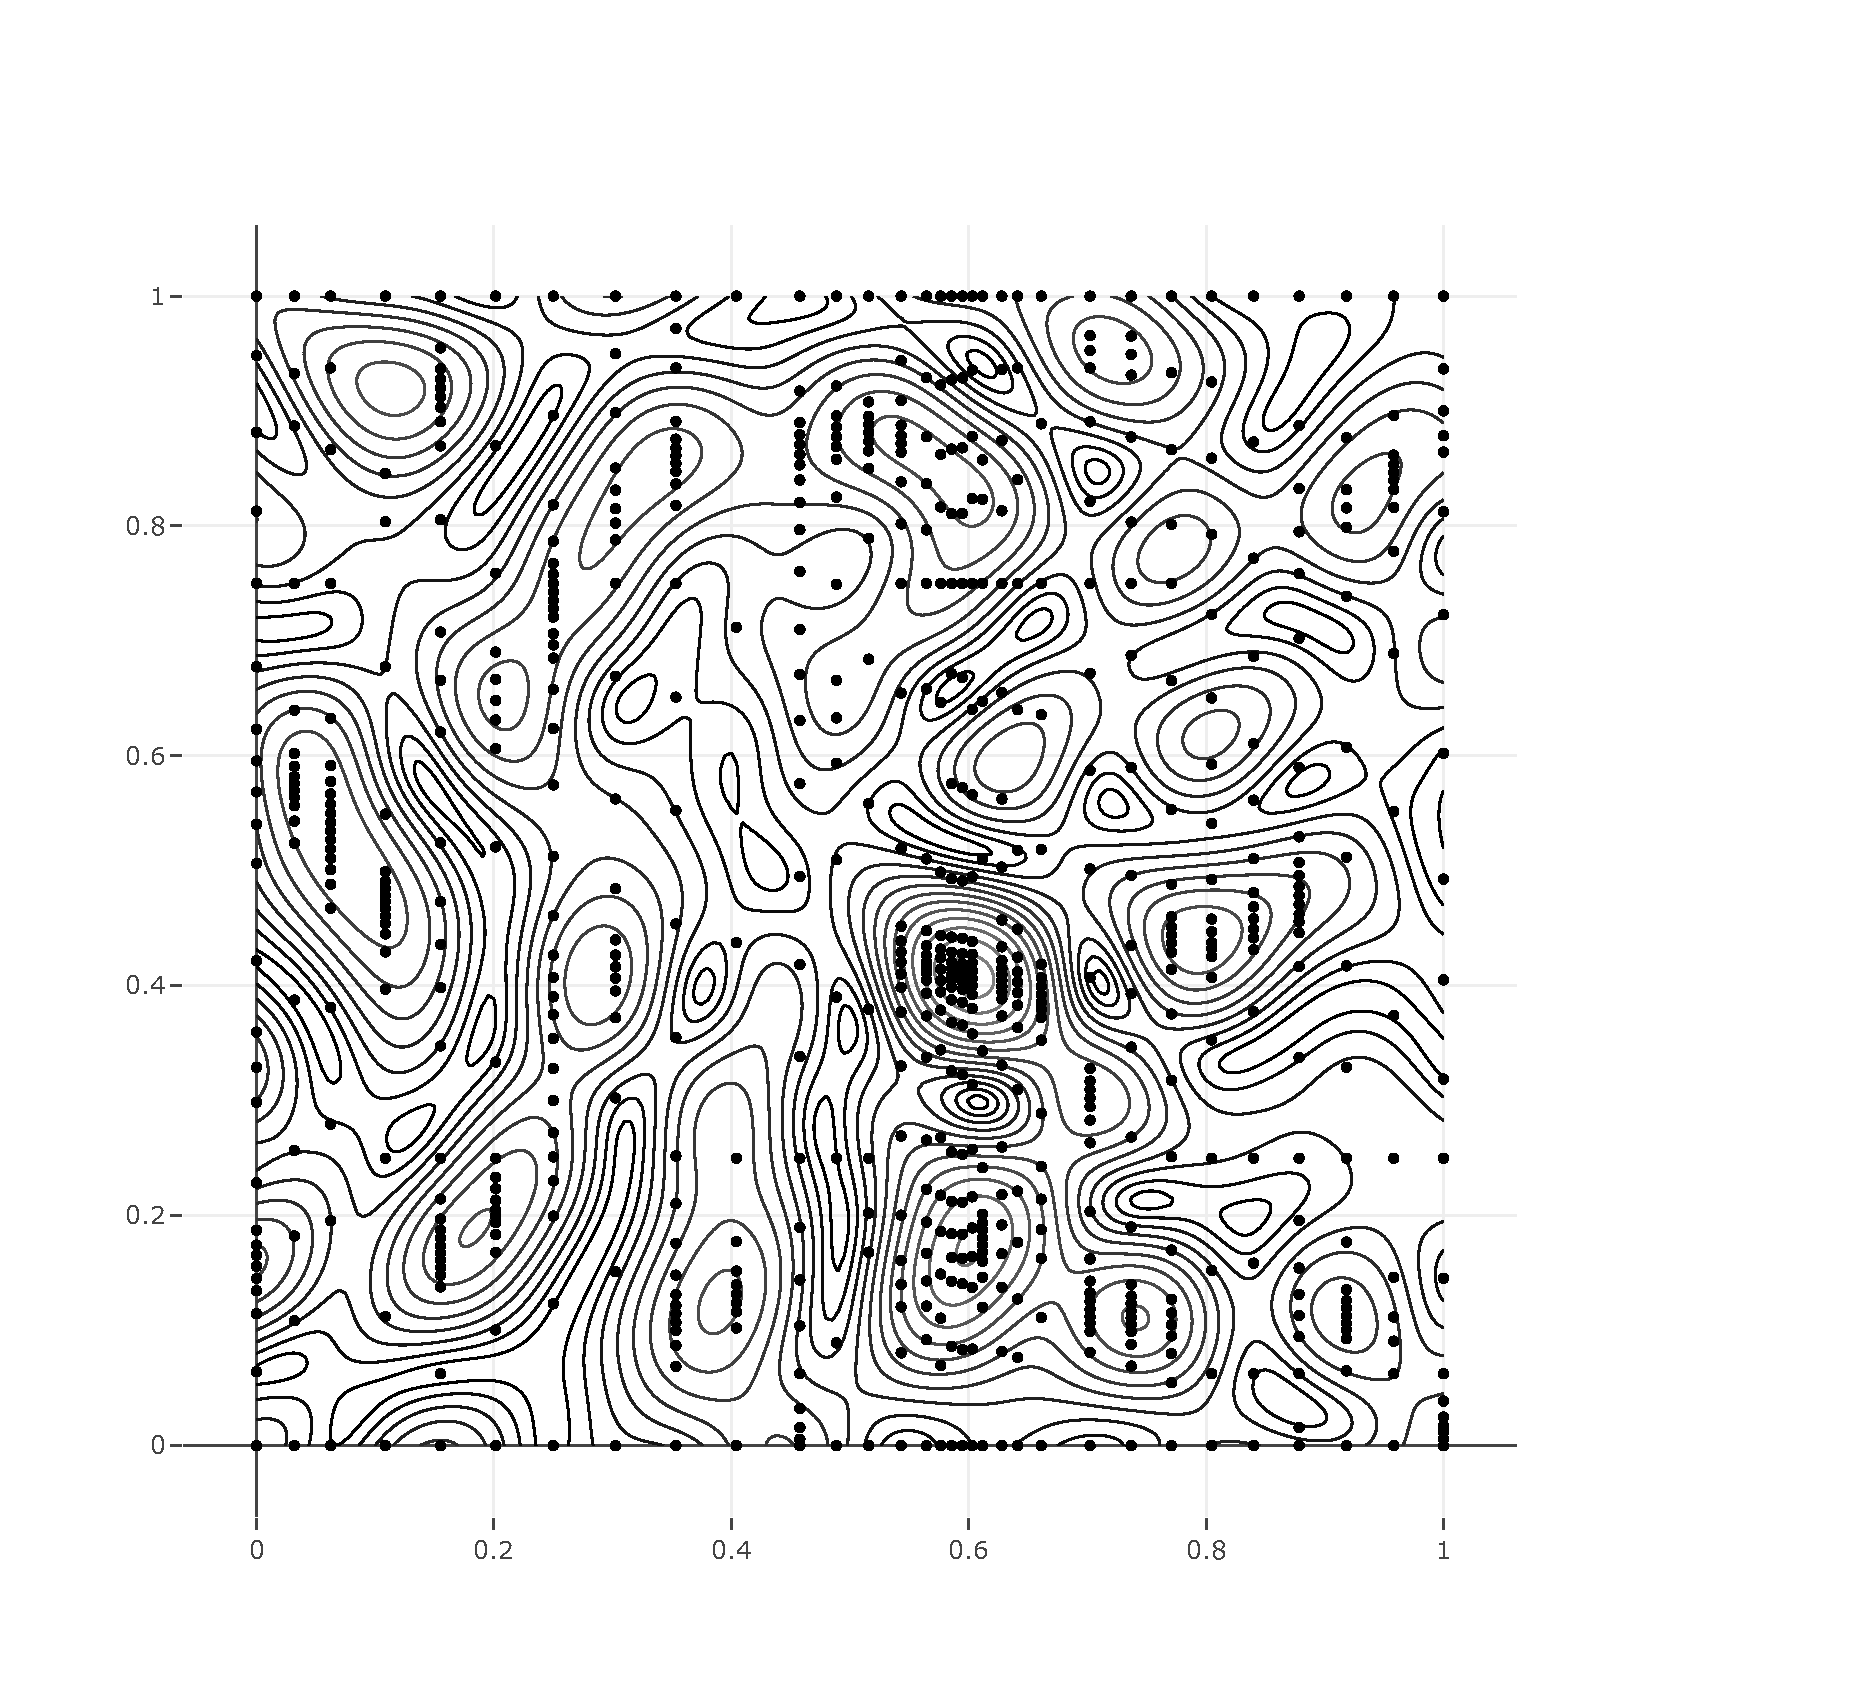
\includegraphics[width=1.1\linewidth]{figures/figure_5_2.pdf}
\caption{Level curves and trial points}
\label{fig:5_2}    
\end{figure}

The nested scheme (\ref{eq:5_18})--(\ref{eq:5_21}) may be generalized in the following way. Let us consider for simplicity a problem (\ref{eq:5_1}) without functional constraints, i.e., $Q=D$, and present the feasible domain  as the direct product of subdomains with smaller dimensions
\begin{displaymath}
D=D_1\times D_2\times\:\ldots\: D_s,\:1\leq s<N,
\end{displaymath}
where the subdomains $D_i,\:1\leq i\leq s,$ are hyperparallelepipeds (\ref{eq:5_3}) of corresponding dimensions $d_i$ such that $1\leq d_i<N$ and $\sum_{i=1}^s{d_i}=N$.

In this case (\ref{eq:5_18}) can be transformed to the form
\begin{displaymath}
\min_{y\in Q}\varphi(y)=\min_{z_1\in D_1}\min_{z_2\in D_2}\ldots\min_{z_s\in D_s}\varphi(y),
\end{displaymath}
where $z_1=u_{\sigma(1)},\:z_i=(y_{\sigma{(i-1)}}+1,\ldots, y_{\sigma(i)}),\:2\leq i\leq s,$ and $\sigma(j)=\sum_{i=1}^j{d_i},\:1\leq j\leq s$.

Then, instead of the family (\ref{eq:5_21}) we can solve the set of nested subproblems 
\begin{displaymath}
\varphi(u_{\sigma(i-1)},z_i)\rightarrow \min,\;z_i\in D_i,
\end{displaymath}
which can be multidimensional with lesser dimensions. Such approach was developed (see \cite{5_BarkGer2014, 5_BarkGerLeb, 5_BarkLeb, 5_SysoyevBarkGerLeb}) in combination of the optimization algorithms based on the Peano space-filling curves for solving the nested multidimensional subproblems.

Moreover, in the family (\ref{eq:5_21}) for several functions $\varphi^i(u_i)$ one can use the operation of taking maximum instead of minimum. In this case it is possible to calculate complex minmax (or maxmin) expressions. 

\section{Properties of one-dimensional subproblems in the nested optimization scheme}
\label{sec:5_2}
While analyzing univariate subproblems (\ref{eq:5_21}) of the nested scheme, two main problems arise:
\begin{description} [a)]
\item [a)] {the necessity to construct the feasible domains $\Pi_i(u_{i-1})$  for the one-dimensional search;}
\item [b)] {it is required to provide the minimization of the one-dimensional functions $\varphi^i(u_{i-1},y_i)$  in the domains  $\Pi_i(u_{i-1})$.}
\end{description}

The structure and the complexity of the projections $\Pi_i(u_{i-1})$  are completely determined by the complexity of the multidimensional feasible domain $Q$. The complexity of the second problem depends on the characteristics of the functions $\varphi^i(u_i)$ . These characteristics are influenced by the properties of the objective function $\varphi(y)$ as well as by the features of the search domain $Q$ defined, in turn, by constraints (\ref{eq:5_2}) and (\ref{eq:5_3}).

\subsection {Structure of the feasible domains of the one-dimensional search}
\label{subsec:5_2_1}
The results of Lemma \ref{lem:5_3}, which has established the equivalence of Definition (\ref{eq:5_9}) and representation (\ref{eq:5_16}) enable to analyze the structure of the domains $\Pi_i(u_{i-1})$. In fact, (\ref{eq:5_16}) provides a constructive apparatus for building the domains $\Pi_i(u_{i-1})$  by means of finding the domains of the non-positivity for the functions $G^i(u_{i-1},y_i)$.

Since the function $G(y)$ is assumed to be continuous in the domain $D$, the functions $G^i(u_i)$ are continuous with respect to $u_i\in D_i$  from (\ref{eq:5_11}) and, therefore, with regard to $y_i\in [a_i,b_i]$  as well. Then, at fixed $u_{i-1}\in D_{i-1}$  each one-dimensional problem (\ref{eq:5_21}) can be rewritten in a unified form
\begin{equation}
\label{eq:5_22}
  \begin{cases}
    \bar{\varphi}(x)\rightarrow\min,\;x\in\bar{Q}\subseteq R^1, \\
    \bar{Q}=\{x\in[a,b]:g(x)\leq 0\},
  \end{cases}
\end{equation}
where the function $g(x)$ is continuous.

The continuity of the constraint $g(x)$ allows one to state that the feasible domain $\bar{Q}$  can be presented as a system of intervals
\begin{equation}
\label{eq:5_23}
\bar{Q}=\bigcup_{j=1}^q{[a^j,b^j]},
\end{equation}
in each of which the function $g(x)$ is non-positive. 

As an example, let us consider the possible cases of the behavior of a continuous function generating the domains of the non-positivity presented in Fig. \ref{fig:5_3}. The corresponding intervals  are marked with  the signs $\times$  on the abscissa axis including the points of tangency. The most right-side interval marked with $\times$ corresponds to the case when the function equals to zero over the interval of non-zero length. 
\begin{figure}[t]
\centering
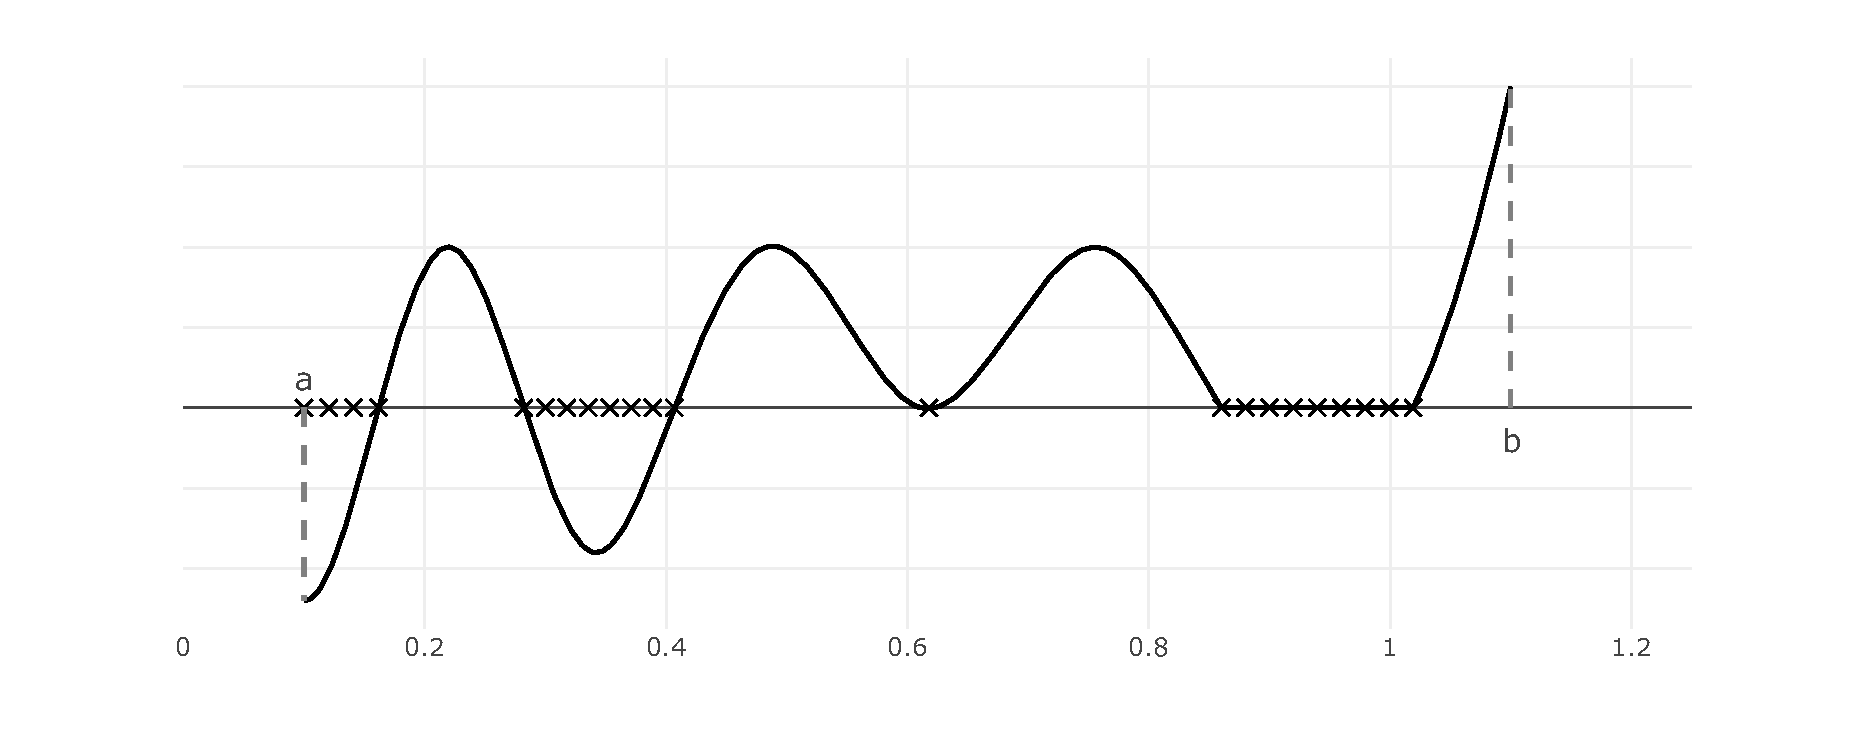
\includegraphics[width=1.1\linewidth]{figures/figure_5_3.pdf}
\caption{Domains of the non-positivity of a continuous function}
\label{fig:5_3}    
\end{figure}
In the system (\ref{eq:5_23}) the number of intervals $q$ can be infinite. As an example of such situation one can consider within the closed interval $[0,1]$ the function
\begin{displaymath}
g(x)=
  \begin{cases}
    x\sin(\frac{1}{x}), & x>0,\\
    0, & x=0.
  \end{cases}
\end{displaymath}

Thus, in the case of a continuous function $G(y)$, the projection $\Pi_i(u_{i-1}$ determined as  (\ref{eq:5_16}) is a set of the kind (\ref{eq:5_23}), i.e.,
\begin{equation}
\label{eq:5_24}
\Pi_i(u_{i-1})=\bigcup_{j=1}^{q_i}{[a_i^j,b_i^j]},
\end{equation}
where, in general, the number of the intervals $q_i$  and their bounds $a_i^j$, $b_i^j$, $1\leq j\leq q_i,$ depend on the vector $u_{i-1}$ , i.e.,
\begin{equation}
\label{eq:5_25}
q_i=q_i(u_{i-1}),\:a_i^j=a_i^j(u_{i-1}),\:b_i^j=b_i^j(u_{i-1}).
\end{equation}

If the domain $Q$  is such that it is possible to obtain the explicit (analytical) expressions for the values $q_i,a_i^j,b_i^j$   as  functions of $u_{i-1})\in Q_{i-1}$  for all $1\leq i\leq N$, then the domain $Q$ is called \textit{the domain with the computable bounds}. In particular, it is possible if all the roots of the functions $G^i(u_{i-1},y_i)$  with regard to the variables $y_i$  can be analytically found.
\begin{example}
\label {exam:5_1}
As the problem to be investigated  the problem (\ref{eq:5_1})--(\ref{eq:5_3}) with 
\begin{equation}
\label{eq:5_26}
  \begin{cases}
    \varphi(y)=y_1^2+y_2^2,\\
   Q=\{y\in D:(y_1-1)^2+(y_2-1)^2-1\leq 0\}, \\
	D=\{y\in R^2:0\leq y_1,y_2\leq 2\}
  \end{cases}
\end{equation}
is considered. The feasible domain is marked with gray in Fig. \ref{fig:5_4}. Also, the level curves of the objective function are shown there. In this problem, the function $G^2(y)=(y_1-1)^2+(y_2-1)^2-1$. It is evident that the function  $G^1(y_1)=\min\{G^2(y_1,y_2):y_2\in [0,\;2]\}=(y_1-1)^2-1$. 
\begin{figure}[t]
\centering
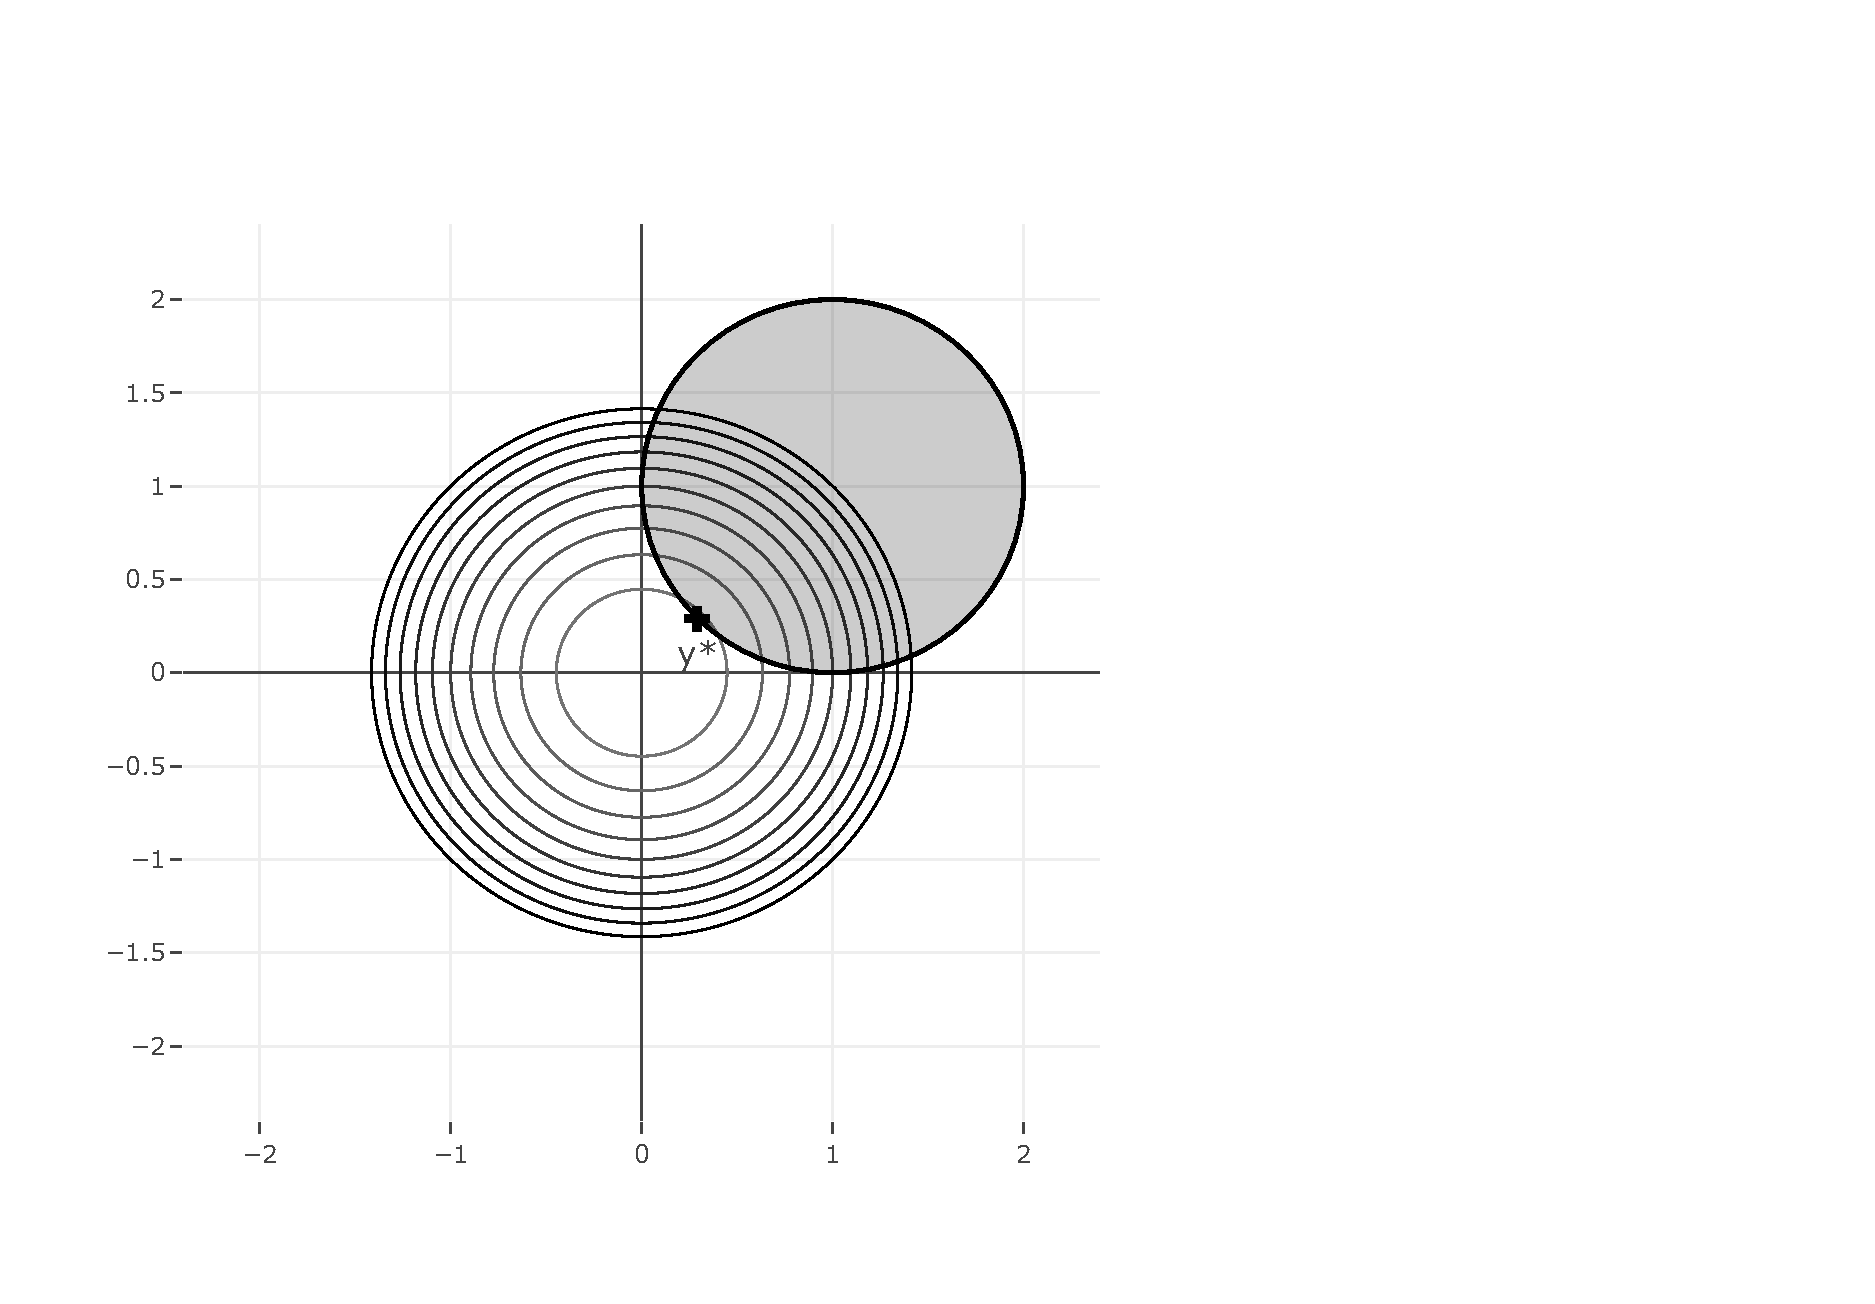
\includegraphics[width=1.1\linewidth]{figures/figure_5_4.pdf}
\caption{Feasible domain and level curves of the objective function}
\label{fig:5_4}    
\end{figure}

According to (\ref{eq:5_16}), the domains where the functions $G^1(y_1)$  for $y_1$  and $G^2(y_1,y_2)$  for $y_2$  are not positive determine the projections $\Pi_1$  and $\Pi_2(y_1)$ , respectively. The domain bounds are the roots of these functions in the interval $[0,2]$. For the function $G^1(y_1)$  these roots are $0$ and $2$. Therefore, $\Pi_1=[0,\:2]$.

The function $G^2(y)=(y_2-1)^2-\alpha^2$, where $\alpha=\sqrt{1-(y_1-1)^2}\leq 1$,  has the roots $1\pm \alpha$ within the interval $[0,2]$ and  it is not positive between these roots. As a result, 
\begin{equation}
\label{eq:5_27}
\Pi_2(y_1)=[1-\sqrt{1-(y_1-1)^2},1+\sqrt{1-(y_1-1)^2}].
\end{equation}

Thus, we can write down the bounds of projections (\ref{eq:5_24}) in an explicit form. Thereby, the domain $Q$ from (\ref{eq:5_26}) is a domain with computable bounds (\ref{eq:5_25}).

The function $\varphi(y)=y_1^2+y_2^2$  is an increasing one for $y_2$  in the interval $[0,2]$. Consequently, it reaches its maximum at the point $1-\alpha$  in the domain (\ref{eq:5_27}), therefore,
\begin{displaymath}
\varphi^1(y_1)=y_1^2+(1-\sqrt{1-(y_1-1)^2})^2=1+2y_1-2\sqrt{1-(y_1-1)^2}.
\end{displaymath}

The first derivative $(\varphi^1(y_1))'=2+\frac{2(y_1-1)}{\sqrt{1-(y_1-1)^2}}$ has a unique root  $y_1^*=1-\frac{1}{\sqrt{2}}$ in the interval  $[0,2]$. 
In addition, the second derivative $(\varphi^1(y_1))''=\frac{2}{(1-(y_1-1)^2)^{3/2}}>0$, therefore, the point $y_1^*=1-\frac{1}{\sqrt{2}}$  gives the minimum value of the function $\varphi^1(y_1)$  equal to $3-2\sqrt{2}$. This value is the sought minimum of the function $\varphi(y)$ in the domain $Q$. 

In order to obtain the coordinate $y_2^*$, which determines the minimum point along with $y_1^*$, let us consider the function $\varphi^2(y_1^*,y_2)$ and find its minimum in the domain $\Pi_2(y_1^*)=[1-\frac{1}{\sqrt{2}},1+\frac{1}{\sqrt{2}}]$, which is obviously achieved at the point $y_2^*=1-\frac{1}{\sqrt{2}}$.

So, the vector $y^*=(1-\frac{1}{\sqrt{2}},1-\frac{1}{\sqrt{2}})$  providing the minimum value $\varphi^*=3-2\sqrt{2}$ of the objective function is the solution of the multidimensional problem (\ref{eq:5_26}). The optimum point is marked with a dark cross in Fig. \ref{fig:5_4}. 
\end{example}

In the example considered above, we have constructed the one-dimensional search domain bounds  analytically by finding the domains of the non-positivity of the corresponding functions $G^i(u_i)$ . At the same time, one can specify a more visual «geometrical» method for the construction of the projections $\Pi_{i+1}(u_i)$. This method follows from definitions (\ref{eq:5_8}) and (\ref{eq:5_9}) and consists in the construction of the sections of the domain $Q$  by planes $u_i=const$. After that, it is necessary to find the bounds of these sections for the coordinate $y_{i+1}$.

In this regard, the following is noteworthy. The computation of the global minimum according to (\ref{eq:5_18}) is analogous to the procedure of computation of a multidimensional integral of the function $\varphi(y)$ over the domain $Q$ by means of the reduction to computing  the recurring (nested) one-dimensional integrals. Here, the domains of the one-dimensional integration are just the corresponding projections $\Pi_i(u_{i-1})$.

As an illustration the example \ref{exam:5_2} can be taken. 
\begin{example}
\label{exam:5_2}
Assume that the domain of the optimization (or of the integration) is defined as
\begin{displaymath}
Q=\{y\in R^2:-4\leq y_1,y_2\leq 4, y_1^2+y_2^2\leq 4,y_1^2+y_2^2\geq 1\}.
\end{displaymath}
\begin{figure}[t]
\centering
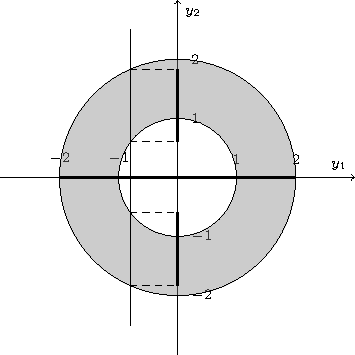
\includegraphics[width=0.8\linewidth]{figures/figure_5_5.pdf}
\caption{Sections and projections}
\label{fig:5_5}    
\end{figure}
In Fig. \ref{fig:5_5} this domain is marked with gray. The left-side line $y_1=const$  generates the section $S_1(y_1)$  as the intersection of the line with the domain $Q$, and the projection  of $S_1(y_1)$  onto the axis $y_2$  determines the projection $\Pi_2(y_1)$ . This projection and the projection $\Pi_1$  are marked with the bold lines in Fig. \ref{fig:5_5}.

These geometrical considerations allow constructing the necessary projections of the problem as 
\begin{displaymath}
\Pi_1=[-2,\:2],
\end{displaymath}
\begin{displaymath}
\Pi_2(y_1)=
  \begin{cases}
    [-\sqrt{4-y_1^2}, \sqrt{4-y_1^2}],\ y_1\in [-2,\:-1]\bigcup [1,\:2],  \\
    [-\sqrt{4-y_1^2}, -\sqrt{1-y_1^2}]\bigcup [\sqrt{1-y_1^2}, \sqrt{4-y_1^2}],y_1\in [-1,\:1].                      	
  \end{cases}
\end{displaymath}
\end{example}

However, finding all roots of a continuous function is a difficult problem, unsolvable analytically, as a rule. In this case, one can try to find these roots numerically. Let us consider, for example, typical problem (\ref{eq:5_22}). In order to find all roots of a continuous function $g(x)$ one can propose  numerical solving  the equivalent optimization problem 
\begin{displaymath}
\left|g(x)\right|\rightarrow \min,x\in [a,b],
\end{displaymath}
which roots of $g(x)$ are the global minima points in. To solve this problem, the characteristical global search algorithms providing the convergence to all global minimum points might be applied.

Another approach to accounting the constraints in the optimization problems (the index method), which does not require to solve any auxiliary problems  is considered in Chapter 4.

The case $Q=D$  when the constraint functions (\ref{eq:5_2}) are absent is an important particular case of the problem (\ref{eq:5_1})--(\ref{eq:5_3}). In this case, $G(y)\equiv 0$ in the domain $D$, and it follows from (\ref{eq:5_12}) that $G^i(u_i)\equiv 0$,$1\leq i\leq N$. Then, according to (\ref{eq:5_16}), 
\begin{displaymath}
\Pi_i(u_{i-1})=[a_i,b_i],
\end{displaymath}
where $a_i,b_i$ are constants.

The optimization domains (\ref{eq:5_2}) can generate projections $\Pi_i(u_{i-1})$  as a single interval for some particular properties of the constraint functions as well. These properties are the convexity of the functions $g_j(y),\:1\leq j\leq m$, providing the convexity of the feasible domain $Q$ and the monotonous unimodality of the constraint functions \cite{5_GrishaginStrongin_EnginCybernetics}, which is more general than the concept of convexity.  In general case, monotonous unimodal constraints can generate non-convex domains $Q$.

In the situation of the monotonous unimodality (or of convexity as a particular case) of the constraints $g_j(y),\:1\leq j\leq m$, the one-dimensional search domains are the intervals 
\begin{displaymath}
\Pi_i(u_{i-1})=[a_i^1(u_{i-1}),b_i^1(u_{i-1})],
\end{displaymath}
the bounds of which, however, are not constant but depend on the vector $u_{i-1}$.
\subsection {Properties of the objective functions in one-dimensional subproblems}
\label{subsec:5_2_2}

The objective function in a subproblem (\ref{eq:5_21}) is the function $\varphi^i(u_{i-1},y_i)$  with fixed $u_{i-1}$ . The character of the dependence of the function $\varphi^i$  on the variable $y_i$  is crucial while solving the subproblems (\ref{eq:5_21}).

Let us consider a class of problems, in which the function $\varphi(y)$ is separable, i.e.,
\begin{equation}
\label{eq:5_28}
\varphi(y)=\sum_{i=1}^N{\varphi_i(y_i)},
\end{equation}
and the constraints $g_j(y)$  are absent, i.e., $Q=D$.

Then, as it follows from (\ref{eq:5_18}) and (\ref{eq:5_28}), 
\begin{displaymath}
\min_{y\in Q}\varphi(y)=\sum_{i=1}^N{\min_{y_i\in [a_i,b_i]}\varphi_i(y_i)},
\end{displaymath}
i.e., to solve the multidimensional problem it is necessary to solve $N$ independent one-dimensional subproblems. For this problem class, the complexity increases linearly with increasing dimensionality. 

Now assume that the function $\varphi(y)$ satisfies the Lipschitz condition with a constant $L>0$ in the domain $Q$, i.e., for any $y',y''\in Q$
\begin{equation}
\label{eq:5_29}
\left|\varphi(y')-\varphi(y'')\right|\leq L\left\|y'-y''\right\|,
\end{equation}
where $\left\|\bullet\right\|$ denotes the Euclidean norm. The obvious question in this case is whether the functions $\varphi^i(u_i)$  satisfy the Lipschitz condition. Generally speaking, it takes place not always.

Let us consider the following example. Assume that two-dimensional objective function $\varphi(y)$  in problem (\ref{eq:5_1})--(\ref{eq:5_3}) satisfies the Lipschitz condition (\ref{eq:5_29}) and the feasible domain  
\begin{displaymath}
Q=\{y\in R^2:y_1^2+y_2^2-1\leq 0\}.
\end{displaymath}

The function $\varphi^2(y)\equiv \varphi(y)$ , obviously, is Lipschitzian with the constant $L$ with regard to the coordinate $y_2$. However, the function $\varphi^1(y_1)$  does not satisfy the condition (\ref{eq:5_29}). As it has been shown in \cite{5_StrMonRus}, this function satisfies the generalized Lipschitz condition (H{\"o}lder condition) in the metric $\rho(y_1',y_1'')=\sqrt{\left|y_1'-y_1''\right|}$  with the constant $L_1=L(1+\sqrt{2})$ , i.e., the inequality 
\begin{displaymath}
\left|\varphi(y_1')-\varphi(y_1'')\right|\leq L_1\sqrt{\left|y_1'-y_1''\right|}.
\end{displaymath}

Sufficient conditions for the Lipschitz property (\ref{eq:5_29})  of functions $\varphi^i(u_i)$  is established by the following theorem (see \cite{5_StrMonRus}).
\begin{theorem}
\label{theor:5_1}
Assume that the function $\varphi(y)$ satisfies the Lipschitz condition (\ref{eq:5_29})  with the constant $L>0$ in a domain $Q$ from (\ref{eq:5_2}) and the bound pairs (\ref{eq:5_27}) are the piecewise linear functions of the kind 
\begin{equation}
\label{eq:5_30}
a_{i+1}(u_i)=\max_{1\leq\nu \leq p_{i+1}}\{\alpha_i^\nu u_i+A_i^\nu\},
\end{equation}
\begin{equation}
\label{eq:5_31}
b_{i+1}(u_i)=\max_{1\leq\nu \leq r_{i+1}}\{\beta_i^\nu u_i+B_i^\nu\},
\end{equation}
where  $\alpha_i^\nu u_i$ and $\beta_i^\nu u_i$ are the scalar products of the vectors from $R^i$  and $A_i^\nu, B_i^\nu$ are constants. Then the functions $\varphi^i(u_i),u_i\in Q_i,$ satisfy the Lipschitz condition with the constants $L_i,1\leq i\leq N,$ 
where
\begin{displaymath}
L_N=L,\:L_i=L\sum_{j=i}^{N-1}{(1+\lambda_j)},\:1\leq i\leq N-1,
\end{displaymath}
\begin{displaymath}
\lambda_j=\max\left\{\max_{1\leq \nu\leq p_{i+1}}\left\|a_j^\nu\right\|,\max_{1\leq \nu\leq r_{i+1}}\left\|b_j^\nu\right\| \right\}.
\end{displaymath}
\end{theorem}

The proof of the theorem is given in \cite{5_StrMonRus}.

Note that the representation of the boundy pairs in the form (\ref{eq:5_30}) and (\ref{eq:5_31}) takes place if the feasible domain is a convex polyhedron. 

If the domain $Q$ is a hyperparallelepiped, all vectors $a_i^\nu,b_i^\nu$ are equal to zero. Therefore, $L_i=L,\:1\leq i\leq N$.

The main conclusion, which follows from the discussion of Lipschitz properties is that the properties of the objective functions of the one-dimensional problems depend essentially not only on the properties of the initial objective function $\varphi(y)$  but also on the shape of the feasible domain $Q$.

In the simplest case, when the domain $Q$ is a hyperparallelepiped all functions $\varphi_i(u_i)$  satisfy Lipschitz condition with the same constant as the function $\varphi(y)$.

If the constraints $g_j(y)$   are piecewise linear convex functions, the Lipschitzness of the functions $\varphi_i(u_i)$  remains but Lipschitz constants for these functions increase in general that worsens the optimization properties of the one-dimensional subproblems.

Finally, the case of the nonlinear constraints can result in the loose of Lipschitzness at all.
\section{Parallel computations for the nested optimization scheme}
\label{sec:5_3}
Applying the parallel methods of the one-dimensional optimization for solving one-dimensional subproblems (\ref{eq:5_21}) in the structure of the nested scheme (\ref{eq:5_18}) enables to obtain a parallel version of the nested scheme with a high degree of variability. For example, one can vary the number of processors employed at different levels of the one-dimensional optimization (i.e., during solving the one-dimensional subproblems for different variables ), apply various parallel one-dimensional optimization methods at different levels, etc.

In order to describe the parallel nested scheme, let us introduce a vector of the parallelization degrees
\begin{equation}
\label{eq:5_32}
\pi=(\pi_1,\pi_2,\:\ldots\:,\pi_N)
\end{equation}
where $\pi_i,1\leq i\leq N$, is the number of one-dimensional subproblems at the $(i+1)$-th recursion level arising as a result of the parallel iterations at the $i$-th level of the one-dimensional optimization and being solved in parallel. The value $\pi_N$  for the coordinate $y_N$  is the number of the parallel trials during the minimization of the function $\varphi^N(y_1,\ldots y_N)\equiv  \varphi(y_1,\ldots y_N)$ with fixed values of $y_1,\ldots, y_{N-1}$, i.e., the number of the objective function values computed in parallel. 

In general, the values $\pi_i,1\leq i\leq N$, may depend on various parameters and may be changed in the course of the optimization. Here, for simplicity, we will consider the case when all components of the vector (\ref{eq:5_32}) are constant. 

The application of the one-dimensional parallel algorithms combined with scheme (\ref{eq:5_18})--(\ref{eq:5_21}) and vector (\ref{eq:5_32}) allows using up to
\begin{displaymath}
P=\prod_{i=1}^N{\pi_i}
\end{displaymath}
processors working in parallel for solving the problem (\ref{eq:5_1})--(\ref{eq:5_3}). Note, the nested scheme generates up to $P/\pi_N$  one-dimensional optimization subproblems being solved simultaneously.

Let us consider, for example, the dimensionality $N=2$. The use of a method with $\pi_1$  parallel trials at one iteration to solve the external univariate problem
\begin{displaymath}
\varphi^1(y_1)\rightarrow\min,y_1\in \Pi_1\subseteq R^1,
\end{displaymath}
generates  $\pi_1$ internal one-dimensional subproblems
\begin{displaymath}
\varphi^2(y_1,y_2)\rightarrow\min,y_2\in \Pi_2(y_1)\subseteq R^1.
\end{displaymath}
Each of these subproblems can be solved by a parallel method with  $\pi_2$  trials at iteration. It means that at the most internal level corresponding  to $i=N$  in (\ref{eq:5_21}) $P=\pi_1\pi_2$  values of the function $\varphi(y)$  are computed, i.e., one can apply $P$  processors running in parallel for computing these values. 

One of possible distributions for   $P=6$ parallel processors is presented in Fig. 
\begin{figure}[t]
\centering
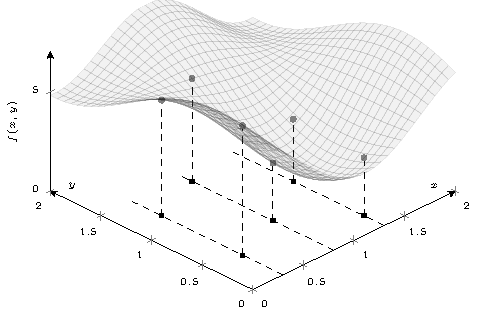
\includegraphics[width=0.8\linewidth]{figures/figure_5_6.pdf}
\caption{Distribution of processors}
\label{fig:5_6}    
\end{figure}

The nested scheme has a significant potential of the parallelization efficiency by means of the use of the asynchronism. This fact is explained by the following reasons.

Let us assume that we combine the nested scheme with a one-dimensional parallel algorithm, which the termination condition differs from realizing a fixed number of iterations in. In this case, the execution time of the trials (the computations of the minimized function) in a parallel iteration at the $i$-th level of the recursion ($1\leq i\leq N-1$)  are different necessarily even if the computation time of the objective function $\varphi(y)$  is independent on the arguments. Remind that the evaluation of the objective function at all levels except the last one consists in solving of a new optimization subproblem.

Assume that the synchronous scheme of the parallel iterations of the one-dimensional optimization algorithm is applied at the $i$-th level of recursion, when the iteration is considered to be complete after execution of all $\pi_i$   trials only. In this case, at least 
\begin{displaymath}
\prod_{j=i+1}^N{\pi_j}
\end{displaymath}
processors, which have already completed solving their subproblems stay idle until the rest subproblems of the $i$-th level are completed. This means that for increasing the productivity of the solving process in the nested scheme it is necessary to use the asynchronous parallel global optimization algorithms, in which the computational resources are used immediately after they become free.

\paragraph{Numerical experiments}

In order to illustrate the theoretical statements, the results of the numerical solving of different multidimensional multiextremal problems are presented below. Three methods which realize multidimensional optimization using the nested scheme (\ref{eq:5_18})--(\ref{eq:5_21}) with combination of information univariate algorithms are considered:
\begin{description} [1)]
\item [1)] {AGSM– algorithm of global search which solves the one-dimensional subproblems inside of the nested scheme by the sequential core information algorithm AGS;}
\item [2)] {PSIM – parallel synchronous information algorithm. It uses AGSIP for solving the one-dimensional subproblems (\ref{eq:5_21});}
\item [3)] {AIPM – asynchronous multidimensional information parallel algorithm applying the asynchronous one-dimensional algorithm proposed in \cite{5_SergGriJCAA} for solving the one-dimensional subproblems.}
\end{description}

The following assumptions are introduced for the first two series of experiments.
\begin{description} [i)]
\item [i)] {The times required for computation of the objective function values are the same for all feasible points. This time can be used as a “unit” time or a “quantum” of time  in the search process. Note, that this assumption is the worst case for the asynchronous method since it is more suitable for the synchronous parallelization.}
\item [ii)] {The time for computation of the objective function value is much greater than the one spent for the implementation of the computational operations of the algorithmic scheme.}
\end{description}

This approach allows abstracting from the architecture of the parallel computational system, on which the experiments were carried out and estimate the «pure» efficiency of the algorithm decision rules. 

Let us denote the time of solving the multidimensional problem (measured in the computational quanta) using the nested reduction scheme with application of the asynchronous algorithm AIPM and the parallelization vector (\ref{eq:5_32}) as $T_A(\pi)=T_A(\pi_1,\pi_2,\ldots,\pi_N)$ , the one with the use of the synchronous algorithm PSIM  (in the analogous conditions) as $T_S(\pi)=T_S(\pi_1,\pi_2,\ldots,\pi_N)$ , and the one with the use of the sequential method AGSM as $T_1=T_S(1,1,\ldots,1)=T_A(1,1,\ldots,1)$ . The last time is simply equal to the number of the computed values of the function $\varphi(y)$.

Furthermore, the numbers of trials performed by the asynchronous method and by the synchronous one will be denoted as $K_A$  and $K_S$, respectively. Using the introduced values, one can define the corresponding time speed-ups achieved owing to the parallelism.

$u_S(\pi)=T_1/T_S(\pi)$ is the speed up of the synchronous algorithm.

$u_A(\pi)=T_1/T_A(\pi)$ is the speed up of the asynchronous algorithm.

As a measure for the comparison of the relative efficiency of the synchronism and the asynchronism one can introduce the coefficient $u(\pi)=u_A(\pi)/u_S(\pi)$.

Note that because of Assumption (i) in the case $\pi=(1,1,\ldots,1,\pi_N)$  we have $u_A(\pi)=u_S(\pi)$ and $u(\pi)=1$.

In the first experiment, the maximization of 100 two-dimensional functions from the class (\ref{eq:3-58}) has been carried out. All experiments were carried out with the precision in the termination criterion $\epsilon=0.01$  and with the reliability parameter $r=2$  for solving all one-dimensional subproblems (\ref{eq:5_21}). All one-dimensional searches have been started from the same starting points {0.2, 0.3, 0.7, 0.8}.

For the method AGSM, which is a pure sequential one, the average number of trials determined as a result of the maximization of 100 functions of the class (\ref{eq:3-58}) was found to be  $T_1= 415.08$. This value can be considered as a measure for the average search time. 

The results for the parallel methods are presented in Table \ref{tab:5_1}.

\begin{table}
\caption{Comparison of the parallel algorithms on the two-dimensional test class}
\label {tab:5_1}
\begin{center}
\begin{tabular}{|c|r|r|r|r|r|}
\hline
$q$ & (2,1) & (2,2) & (2,3) & (2,4) & (2,5)   \\
\hline
$\ \ $$K_A\ \ $  &  $\ \ \ $409.46 & $\ \ \ $397.96 & $\ \ \ $419.41 & $\ \ \ $456.00 & $\ \ \ $510.60  \\
\hline
$K_S$  & 413.89 & 409.24 & 424.08 & 458.60 & 514.20  \\
\hline
$T_A$  & 204.73 &  99.49 &  69.90 &  57.00 &  51.06  \\
\hline
$T_S$  & 234.52 & 114.63 &  77.79 &  62.46 &  56.89  \\
\hline
$u_A$  &   2.03 &   4.17 &   5.94 &   7.28 &   8.13  \\  
\hline
$u_S$  &   1.77 &   3.62 &   5.34 &   6.64 &   7.30  \\
\hline
$u$    &   1,15 &   1,15 &   1,11 &   1,10 &   1,23  \\
\hline
\hline
$q$ & (3,1) & (3,2) & (3,3) & (3,4) & (3,5)   \\
\hline
$K_A$  & 427.23 & 429.18 & 432.90 & 472.20 & 529.95  \\
\hline
$K_S$  & 432.40 & 426.16 & 433,83 & 469.44 & 527.90  \\
\hline
$T_A$  & 123.41 &  71.53 &  48.10 &  39.35 &  35.33  \\
\hline
$T_S$  & 174.38 &  84.90 &  55.95 &  44.63 &  40.62  \\
\hline
$u_A$  &   2.91 &   5.80 &   8.63 &  10.55 &  11.75  \\
\hline
$u_S$  &   2.38 &   4.89 &   7.42 &   9.30 &  10.22  \\
\hline
$u$    &   1.22 &   1.19 &   1.16 &   1.13 &   1.15  \\
\hline
\hline
$q$ & (4,1) & (4,2) & (4,3) & (4,4) & (4,5)   \\
\hline
$K_A$  & 459.88 & 447.12 & 469.32 & 494.40 & 565.20  \\
\hline
$K_S$  & 458.09 & 459.38 & 466.44 & 502.08 & 570.70  \\
\hline
$T_A$  & 114.97 &  55.89 &  39.11 &  30.90 &  28.26  \\
\hline
$T_S$  & 144.45 &  71.38 &  46.58 &  36.92 &  33.69  \\
\hline
$u_A$  &   3.61 &   7.43 &  10.61 &  13.43 &  14.69  \\
\hline
$u_S$  &   2.87 &   5.82 &   8.91 &  11.24 &  12.32  \\
\hline
$u$    &   1.26 &   1.28 &   1.19 &   1.19 &   1.19  \\
\hline
\end{tabular}
\end{center}
\end{table}
The next series of the experiments consists in the minimization of the multidimensional function \cite{5_LucidiPiccioni}
\begin{equation}
\label{eq:5_33}
\varphi(y)=\frac{\pi}{N}\left\{10\sin^2(\pi y_1)+(y_N-1)^2+\sum_{i=1}^{N-1}{[(y_i-1)^2)(1+10\sin^2(\pi y_{i+1})]}    \right\}
\end{equation}
where $-2\leq y_i\leq 4,\;1\leq i\leq N$, for the dimensions $N=$ 3, 4, and 5. The precision $\epsilon=0.12$ and the reliability parameter $r = 2$ were used in all the experiments. At the initial search steps the first four trials were conducted at the points {-1.2, -0.5, 0.0, 2.2} in all one-dimensional subproblems (\ref{eq:5_21}). The results of the computations for the parallel algorithms are presented in Table \ref{tab:5_2}.
\begin{table}
\caption{Comparison of the parallel algorithms for the functions (\ref{eq:5_33}) of various dimensions}
\label {tab:5_2}
\begin{center}
\begin{tabular}{|c|c|c|c|c|c|}
\hline
\multirow{8}{*}{$N=3$} & $q$ & (1,1,1) & (2,2,2) & (3,3,3) & (4,4,4) \\
\cline{2-6}
		& $K_A$ &  7 791  &  7 056  &  7 884  &  10 368   \\
\cline{2-6}
		& $K_S$ &  7 791  &  6 772  &  7 548  &  10 836   \\
\cline{2-6}
		& $T_A$ &  7 791  &   882  &   292  &    162   \\	
\cline{2-6}
		& $T_S$ &  7 791  &  1 013  &   390  &    216   \\		
\cline{2-6}
		& $u_A$ &  1.00  &  8.83  & 26.68  &  48.09   \\
\cline{2-6}
		& $u_S$ &  1.00  &  7.69  & 19.98  &  36.07   \\
\cline{2-6}
		& $u$   &  1.00  &  1.15  &  1.34  &   1.33   \\
\hline
\hline
\multirow{8}{*}{$N=4$} & $q$ & (1,1,1,1) & (2,2,2,2) & (3,3,3,3) & (4,4,4,4) \\  
\cline{2-6}
		& $K_A$ &  155 694  &  136 576  &  165 807  &  201 216   \\
\cline{2-6}
		& $K_S$ &  155 694  &  130 168  &  152 895  &  232 682   \\
\cline{2-6}
		& $T_A$ &  155 694  &  8 536  &   2 047  &   786   \\	
\cline{2-6}
		& $T_S$ &  155 694  & 10 658  &  3 062  &    1 296   \\		
\cline{2-6}
		& $u_A$ &  1.00  & 18.24  & 76.06  & 198.08   \\
\cline{2-6}
		& $u_S$ &  1.00  & 14.61  & 50.85  & 120.13   \\
\cline{2-6}
		& $u$   &  1.00  &  1.25  &  1.50  &   1.65   \\
\hline
\hline
\multirow{8}{*}{$N=5$} & $q$ & (1,1,1,1,1) & (2,2,2,2,2) & (3,3,3,3,3) & (4,4,4,4,4) \\  
\cline{2-6}
		& $K_A$ &  3111771  &  2635872  &  3258144  &  4786176   \\
\cline{2-6}
		& $K_S$ &  3111771  &  2502128  &  3097143  &  4996416   \\
\cline{2-6}
		& $T_A$ &  3111771  &  82371  &   13408  &   4674   \\	
\cline{2-6}
		& $T_S$ &  3111771  & 112485  &  24119  &    7776   \\		
\cline{2-6}
		& $u_A$ &  1.00  & 37.78  & 232.08  & 665.76   \\
\cline{2-6}
		& $u_S$ &  1.00  & 27.66  & 129.02  & 400.18   \\
\cline{2-6}
		& $u$   &  1.00  &  1.36  &  1.80  &   1.67   \\
\hline
\end{tabular}
\end{center}
\end{table}

In the next series of experiments, the function computation time was assumed to depend on the trial point. Problem (\ref{eq:5_33}) was considered for  $N=3$; the precision of the method $\epsilon=0.01$ and the reliability parameter $r=2$ were taken. In all one-dimensional subproblems (\ref{eq:5_21}) the first four trials were conducted at the points {-1.2, -0.5, 0.0, 2.2}. The two kinds of the dependencies $t(y)$ of the function value computation time per one trial point were used. In experiment A
\begin{displaymath}
t_1(y)=\left\lfloor 999\frac{\varphi(y)-\varphi_{min}}{\varphi_{min}-\varphi_{max}}\right\rfloor,
\end{displaymath}
where $\left\lfloor x\right\rfloor$  is the integer part of $x$, $\varphi_{min}=0$, $\varphi_{max}=185$, and in experiment B
\begin{displaymath}
t_2(y)=1000-t_1(y)
\end{displaymath}
were used.

Table 5.3 contains the results of the experiments A and B.
\begin{table}
\caption{Comparison of parallel algorithms in the case of variable time of trial execution}
\label {tab:5_3}
\begin{center}
\begin{tabular}{|c|c|c|c|c|}
\hline
 & \multicolumn{2}{c|}{Experiment A} & \multicolumn{2}{c|}{Experiment B} \\
\hline
$q$ & (2,2,2) & (3,3,3) & (2,2,2) & (3,3,3)    \\
\hline
$K_A$ & 106 802 & 117 270 & 105 599 & 111 774 \\
\hline
$K_S$ & 101 510 & 103 671 & 101 510 & 103 671 \\
\hline
$T_A$ & 738 361 & 221 739 & 11 900 017 & 3 629 895 \\
\hline
$T_S$ & 1 527 229 & 791 559 & 16 943 876 & 5 769 930 \\
\hline
$u$   & 2.07  &  3.57  &  1.42  &  1.59  \\
\hline
\end{tabular}
\end{center}
\end{table}

It results from Table \ref{tab:5_3} that both the methods make a small number of redundant trials only, and the asynchronous algorithm is faster than the synchronous one.

Now let us consider a parallel characteristical algorithm. It is possible construct its generalization onto the synchronous and asynchronous cases like it has been done in Chapter 3 and compare the speed-ups of these versions as a measure of parallelization efficiency. This approach allows estimating the potential of various parallelization schemes of the algorithm decision rules. In the framework of this approach, the experiments were carried out for core information global search algorithm (\ref{eq:2_36})--(\ref{eq:2_38}) for the  class of functions of various dimensionality. The average values of $u_S(\pi)$ and $u_A(\pi)$ obtained by the optimization of 100 multiextremal two-dimensional functions selected randomly from the test class (\ref{eq:2-58}) are presented in Fig. \ref{fig:5_7}. 
\begin{figure}[t]
\centering
%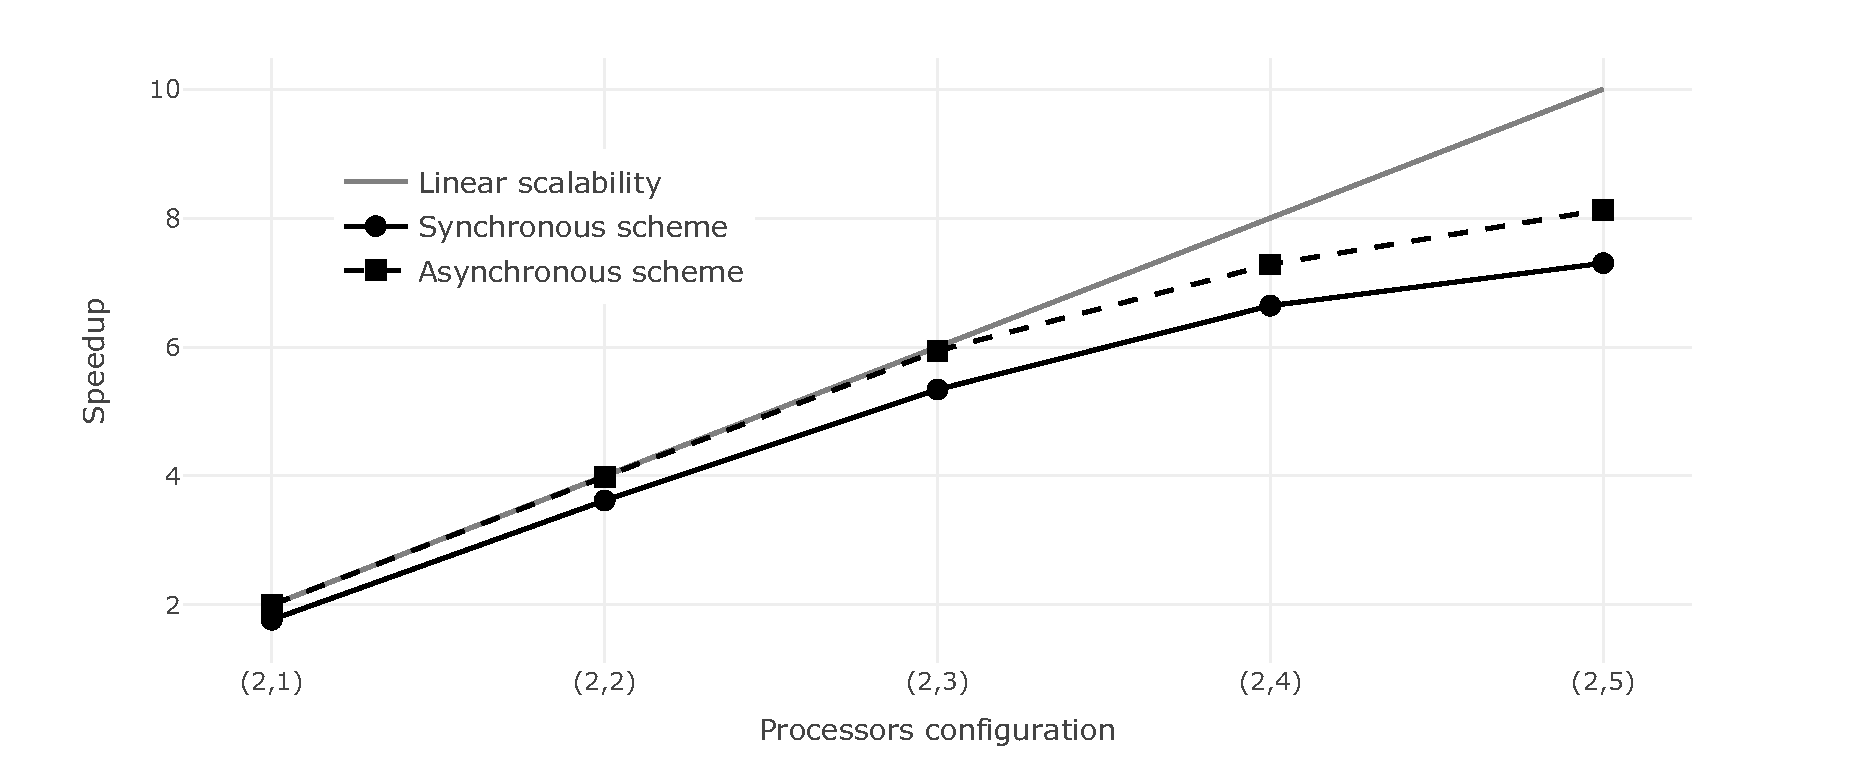
\includegraphics[width=0.8\linewidth]{figures/figure_5_7.pdf}
\caption{Comparative speed-ups of the synchronous scheme and of the asynchronous one on the two-dimensional test function class}
\label{fig:5_7}    
\end{figure}
The function plots demonstrate the dependencies of the speed up (the ordinate axis) on parallelization vector (\ref{eq:5_32}), the variants of which are shown on the abscissa axis. The upper plot corresponds to the «ideal» speed up. The middle and the lower plots reflect the speed-ups of the asynchronous scheme and of the synchronous one, respectively. 

An analogous graph for the case of the optimization of a multiextremal five-dimensional function
\begin{displaymath}
\varphi(y)=\frac{\pi}{5}\left(\sin^2(\pi y_1)+5(y_5-1)^2+\sum_{i=1}^4{[(y_i-1)^2)(1+10\sin^2(\pi y_{i+1})]}    \right)
\end{displaymath}
is presented in Fig. \ref{fig:5_8}. For the one-dimensional optimization the parallel version of the broken lines method (\ref{eq:2_36}), (\ref{eq:2_37}) with the adaptive estimate of Lipschitz constant (\ref{eq:2_39}), (\ref{eq:2_40}) was used.
\begin{figure}[t]
\centering
%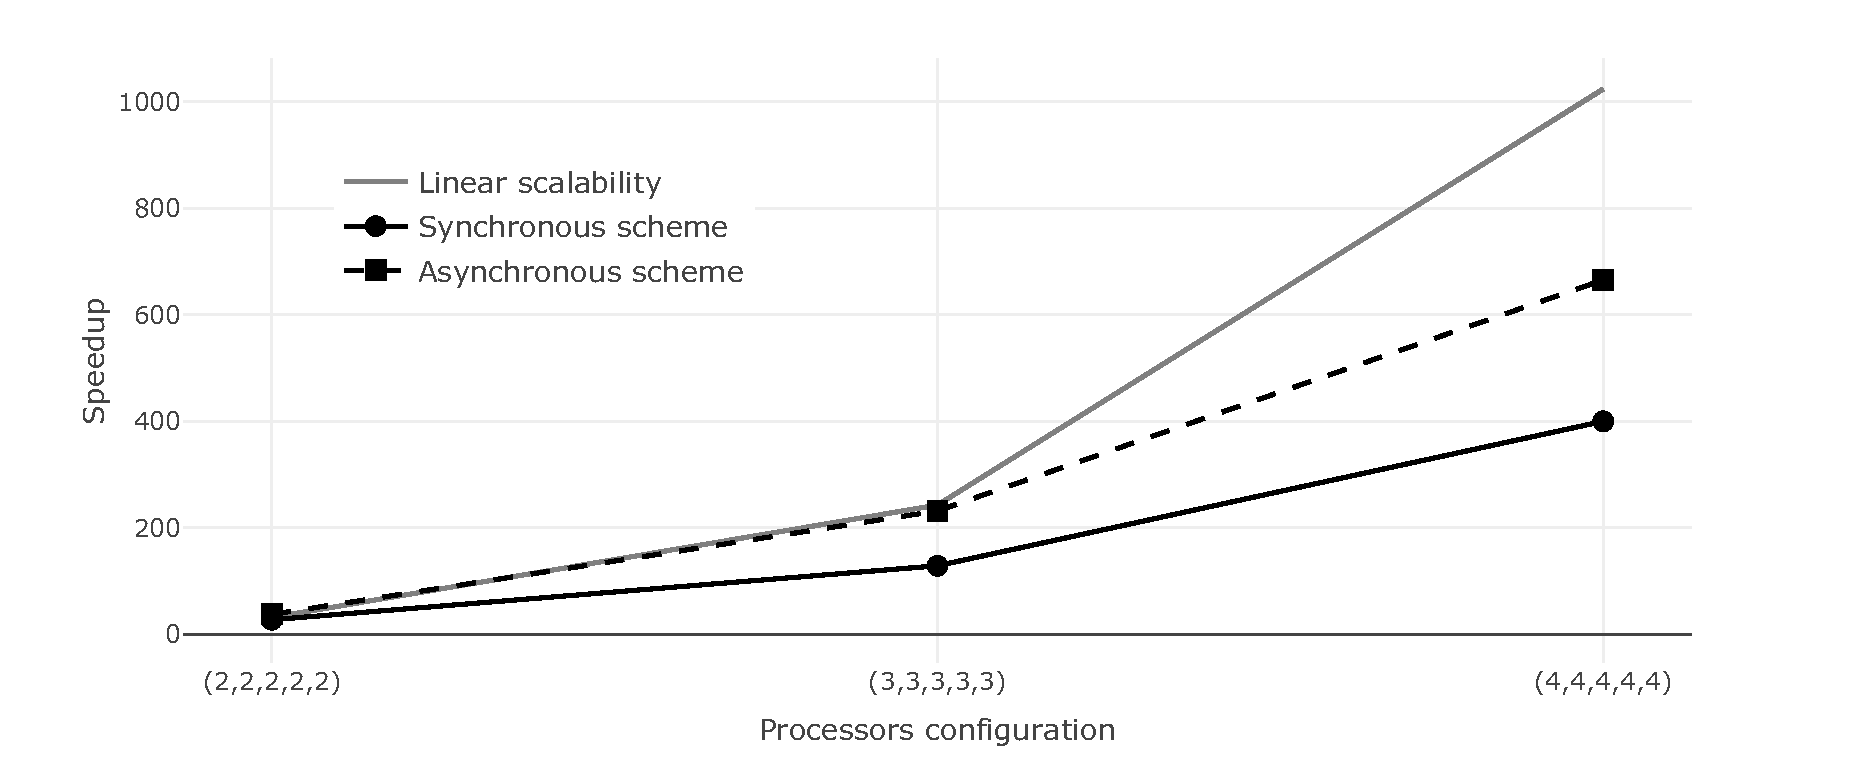
\includegraphics[width=0.8\linewidth]{figures/figure_5_8.pdf}
\caption{Speed-ups of the synchronous and asynchronous broken lines method}
\label{fig:5_8}    
\end{figure}

As in the previous case, the upper plot corresponds to the «ideal» speed up. The middle and lower plots reflect the speed-up of the asynchronous scheme and of the synchronous one, respectively. 
\section{Adaptive nested scheme of dimensionality reduction}
\label{sec:5_4}
\subsection {General description}
\label{subsec:5_4_1}
The univariate subproblems of the family (\ref{eq:5_21}) are generated recursively and it is possible to describe their connections using a hierarchical structure “tree” in which  the root is the subproblem (\ref{eq:5_19}) and the leaves are the subproblems (\ref{eq:5_20}). An example of the full subproblems’  tree (obtained after completion of solving all the family (\ref{eq:5_21})) for the dimension $N=3$  is shown in Fig. \ref{fig:5_9}.
\begin{figure}[ht]
\centering
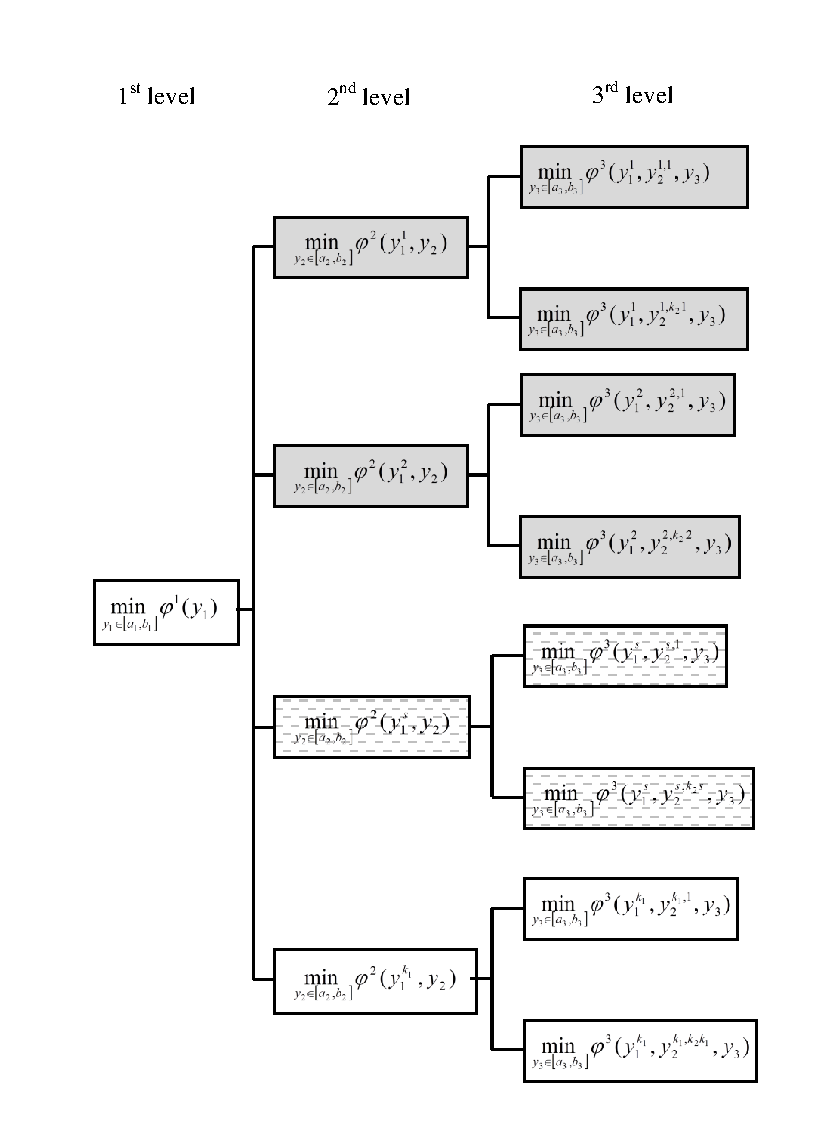
\includegraphics[width=1.0\linewidth]{figures/figure_5_9.pdf}
\caption{Tree of subproblems in the nested optimization scheme}
\label{fig:5_9}    
\end{figure}

In the classical implementation of the nested scheme there are some important features. Namely, execution of any trial in a subproblem at the level $i<N$ generates a sub-tree of the general tree (the execution of a trial in a subproblem at the level $i=N$ consists in computation of the objective function $\varphi(y)$ from (\ref{eq:5_1})). For example, in the root subproblem (\ref{eq:5_19})  the trial at the point $y_1^s$  requires solving univariate subproblems of the sub-tree marked in Fig.\ref{fig:5_9} with the background as the dashed lines. Moreover, until the subproblems of this sub-tree will be completely solved no new trial can be initiated in the root subtask. As a consequence, while solving the subproblems belonging to the dashed sub-tree the subproblems corresponding to the other sub-trees either have been solved already (they are marked in Fig \ref{fig:5_9} with grey) or will be solved later (marked with no background).

As it follows from the presented structure the subproblems at the same level are solved independently and the search information obtained by a subproblem is not used in the other subproblems at this level (and, of course, in all sub-trees generated them).  Such loss of information leads to increasing the number of trials and slows up the optimization process. 

To overcome this drawback in the paper \cite{5_GerGriGer} a new version of the nested optimization scheme in which the other way of solving the univariate subproblems has been proposed. In this version called adaptive nested optimization scheme instead of the strictly subordinated order of solving the univariate subproblems the principle of simultaneous consideration of all subproblems arising dynamically is used. The adaptive scheme does not require to solve each  one-dimensional subproblem  up to the end and all the generated subproblems participate in the multidimensional optimization at any iteration of its realization. The main principle of such realization is close to the idea of characteristical algorithms. Namely, to each subproblem a numerical value called its characteristic is assigned and the multidimensional iteration consists in the choice of the subproblem with maximal characteristic and performing a new trial in this subtask. If the characteristics are assigned in such a way that they take into account the values of functions minimized in subproblems following the principle “low values influence increasing the characteristic” then the subproblems with lower values will be chosen more often than the subproblems with the higher ones and computational resources will not be spent for solving the latters unlike the classical nested scheme where these subproblems have to be solved completely. 

The detailed algorithmic implementation of the adaptive nested scheme can be found in \cite{5_GerGriGer}. Here we give a description of this scheme in a general form.

\textbf{Start stage.}

Create in some way an initial set $S$  of subproblems (\ref{eq:5_21}) including a few subproblems at each level of recursion.
\begin{description} [\textbf{Step G1.}]
\item [\textbf{Step G1.}] {Juxtapose to each subproblem from the set $S$ a numerical value called characteristic of this problem.}
\item [\textbf{Step G2.}] {Choose the subproblem with the greatest characteristic (the currently best subproblem).}
\item [\textbf{Step G3.}]{Compute a new trial point in the chosen subproblem.}
\item [\textbf{Step G4.}]{Build the sub-tree of subtasks generated by this trial point in accordance with the nested scheme  (\ref{eq:5_18})--(\ref{eq:5_21}) and add new subproblems to the set $S$.}
\item [\textbf{Step G5.}]{If the termination  criterion is fulfilled in the root subproblem (\ref{eq:5_19}) stop the search and take as a result of optimization the least computed value of the objective function $\varphi(y)$ and its coordinates as the global minimizer. Otherwise, go to \textbf{Step G1}.}
\end{description}

The crucial question arising in the general scheme is how to choose characteristics of the subproblems.  A possible way can be suggested if for solving the subproblems (\ref{eq:5_21}) a one-dimensional characteristical algorithm is used. In this case as the characteristic of the subtask one can take the best interval characteristic (\ref{eq:2_31}) of this method. Moreover, as a stopping criterion of the multidimensional search the termination criterion (\ref{eq:2_21}) in the root problem (\ref{eq:5_19}) can be taken, i.e., the multidimensional optimization is stopped when the interval with the maximal characteristic in the subproblem (\ref{eq:5_19}) becomes less than predefined accuracy. 

For realization of this idea the core information  algorithm AGS (\ref{eq:2_37})--(\ref{eq:2_39}) can be taken. Theorem ~\ref{theor:5_2} gives the theoretical substantiation of convergence to global minimum for the adaptive nested scheme combined with AGS for solving internal univariate subproblems (\ref{eq:5_21}).

Before formulating the theorem let us introduce a few notations. First of all, it is necessary to pay attention that during realization of the adaptive scheme the values of objective functions   in subproblems (\ref{eq:5_21}) for $1\leq i\leq N-1$   are evaluated approximately, as for obtaining the exact value $\varphi^i(u_{i-1},\tilde{y_i})$ at a 
point  $\tilde{y_i}$  it is required to minimize exactly the function $\varphi^{i+1}(u_{i-1},\tilde{y_i},y_{i+1})$  
at the next level of recursion. So, instead of exact values  $\varphi^i(u_{i-1},y_i^q),\:1\leq q\leq k_i$,   at trial 
points $y_i^1,\ldots,y_i^{k+i}$  we have the values  $\psi^i(u_{i-1},y_i^q),\:1\leq q\leq k_i$,  such that 
\begin{equation}
\label{eq:5_34}
\left|\varphi^i(u_{i-1},y_i^q)-\psi^i(u_{i-1},y_i^q)\right|\leq \gamma_q^i,1\leq q\leq k_i,
\end{equation}
where $\gamma_q^i$ can be interpreted as errors of evaluations for the exact values $\varphi^i(u_{i-1},y_i^q)$, $1\leq q\leq k_i$. As a consequence, after termination of the multidimensional optimization instead of global minimum $\varphi^*$  of the function (\ref{eq:5_1})  there is an approximate estimate $\psi^*$ of it. In this regard the question on the proximity of values $\varphi^*$ and  $\psi^*$ is very important. The answer gives the following theorem (see \cite{5_GerGriGer}).
\begin{theorem}
\label{theor:5_2}
Let the problem (\ref{eq:5_1})--(\ref{eq:5_3}) be considered without functional constraints (\ref{eq:5_2}), i.e., the admissible domain $Q$ coincides with the hyperparallelepiped $D$, and in the adaptive scheme  the information algorithm AGS (\ref{eq:2_37})--(\ref{eq:2_39}) be applied for one-dimensional optimization (\ref{eq:5_21}). If
\begin{enumerate}
\item {the objective function $\varphi(y)$  of the problem (\ref{eq:5_1}) satisfies in the domain $D$  the Lipschitz condition (\ref{eq:5_29}) with a finite constant $L>0$;}
\item {during solving the subproblems (\ref{eq:5_21}) the parameter $m$ from (\ref{eq:2_39}) satisfies the inequality $m>2L$;}
\item {while solving the root problem (\ref{eq:5_19}) the termination criterion (\ref{eq:2_21}) is used with $\epsilon=0$;}
\item {for any function $\varphi^i(u_{i-1},y_i)$  of the family (\ref{eq:2_21}) the conditions 
\begin{equation}
\label{eq:5_35}
\gamma_{\tau-1}^i+\gamma_\tau^i\leq 2\varphi(y^*)+L(y_i^\tau-y_i^{\tau-1})--(\varphi(u_{i-1},y_i^{\tau-1}+\varphi(u_{i-1},y_i^\tau)
\end{equation}
hold for the computational errors $\gamma_{\tau-1}^i,\gamma_\tau^i$  of trials at the adjacent points $ y_i^{\tau-1},y_i^\tau$ such that
\begin{displaymath}
y_i^{\tau-1}\leq y_i^*\leq y_i^\tau,
\end{displaymath}
where $y^*=(y_1^*,\ldots,y_N^*)$  is the global minimizer of the problem (\ref{eq:5_1})--(\ref{eq:5_3}),}
\end{enumerate}
then the sequence of multidimensional trials generated by the adaptive scheme converges to the global minimizer $y^*$ .
\end{theorem}

This theorem provides sufficient conditions of convergence to global minimum for the adaptive scheme in the combination with the method AGS. The proof of the theorem can be found in \cite{5_GerGriGer}. Analogous theorem for the adaptive nested scheme with combination of the univariate broken lines method \cite{5_Piyavskij} has been given in \cite{5_GriIsrSergAMC}.
\subsection {Numerical experiments}
\label{subsec:5_4_2}
To demonstrate the efficiency of the adaptive nested scheme let us consider a function from the 2-dimensional test class (\ref{eq:3-58}) (see \cite{5_GrishaginOperChar, 5_StrSergMon2000}). In Fig.~\ref{fig:5_10} the level curves of this function and distribution of trials (marked by points) are presented. The left panel corresponds to the adaptive scheme and the right panel to the classical one. For optimization of the function these schemes are used in combination with the method AGS for solving the univariate subproblems (\ref{eq:5_21}). In both the cases the method parameter $r=3$  and the search accuracy $\epsilon=0.01$ in termination criterion (\ref{eq:2_21}) were used.
\begin{figure}[ht]
\centering
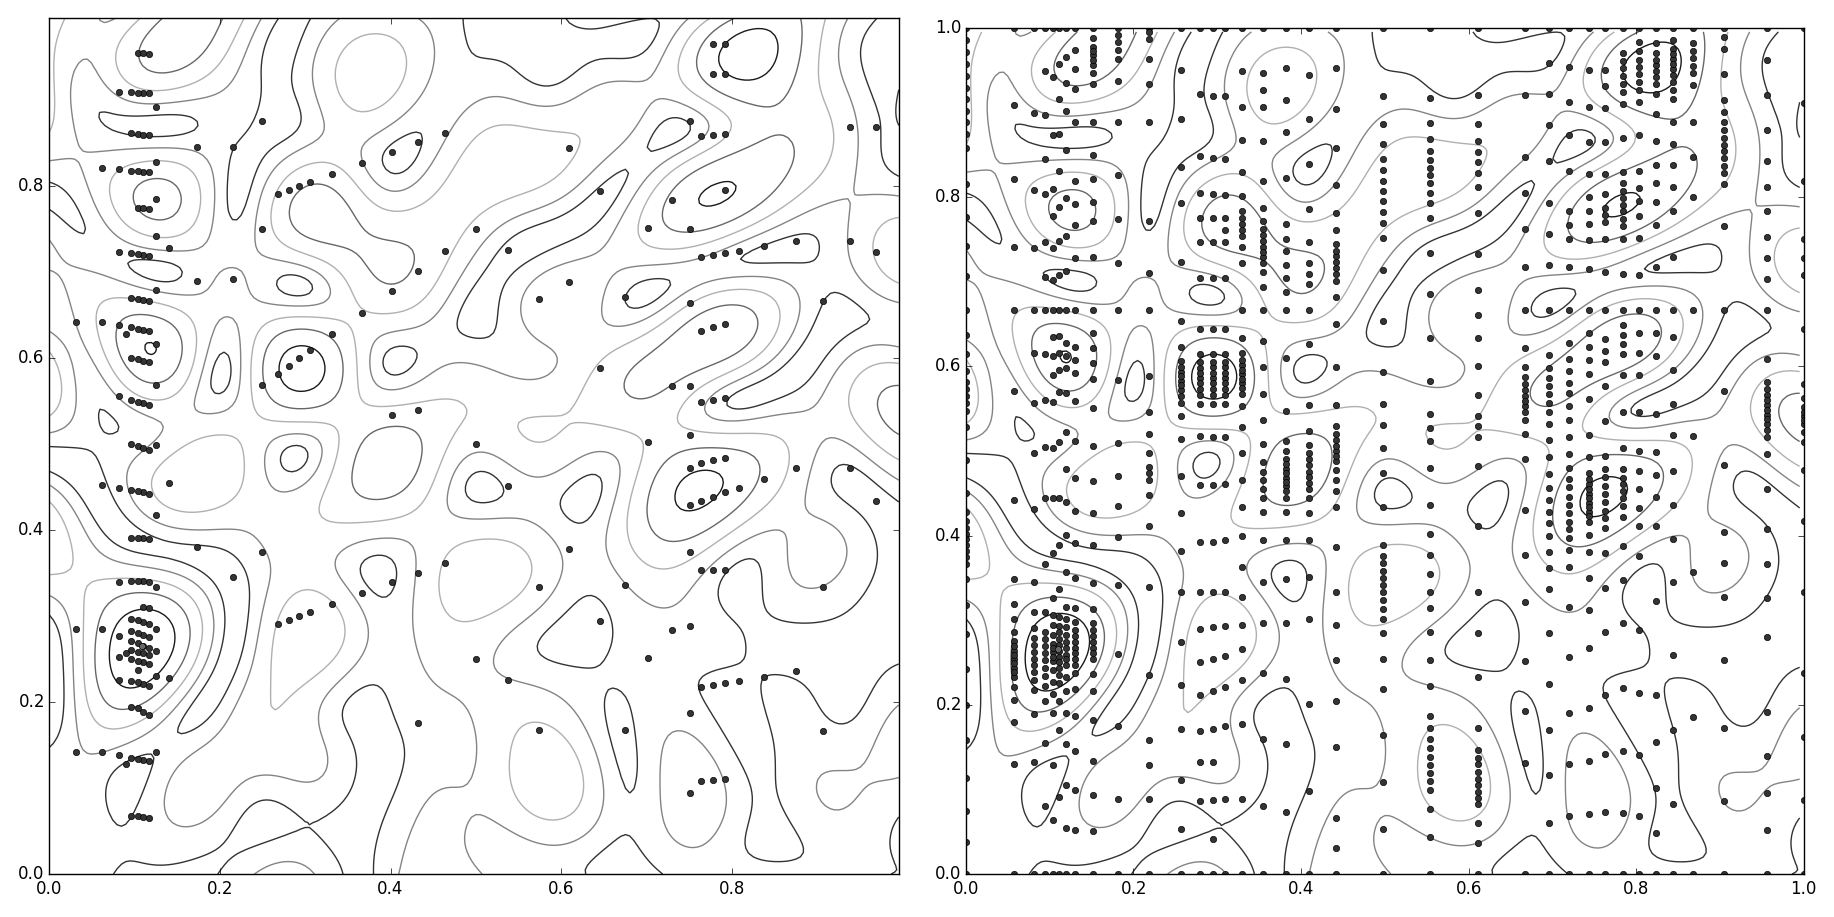
\includegraphics[width=1.0\linewidth]{figures/figure_5_10.png}
\caption{Trials distribution of the adaptive scheme (the left panel) and of the classical one (the right panel).}
\label{fig:5_10}    
\end{figure}

Both the schemes have provided the required accuracy of the problem solution. However, the adaptive scheme has spent significantly less trials, namely, the classical scheme evaluated the objective function 1139 times while the adaptive version carried out 257 trials only.

Another experiment was executed \cite{5_GriIsrSergAMC} on the set of 100 three-dimensional functions belonging to the well-known test class GKLS \cite{5_GavianoKvasovLeraSergeyev}. The GKLS parameters of the test functions were as follows:
\begin{itemize}
\item {10 local minima;}
\item {standard function value $-1.0$ at the  global minimizer;}
\item{distance 0.9 from the global minimizer to the vertex of the paraboloid;}
\item{radius 0.12 of the attraction region of the global minimizer.}
\end{itemize}

The following algorithms were compared by means of the method of operational characteristics – the adaptive nested scheme (AGS-A) and the classical nested scheme (AGS-C) with the univariate method AGS inside of both the schemes, and the very popular method DIRECT \cite{5_Jones, 5_JonesPerttunenStuckman} as an example of global optimization methods of different nature. 
Operational characteristics (see Subsection ~\ref{subsec:2_2_3} of Chapter 2) of the methods compared are presented in Fig. ~\ref{fig:5_11}.
\begin{figure}[ht]
\centering
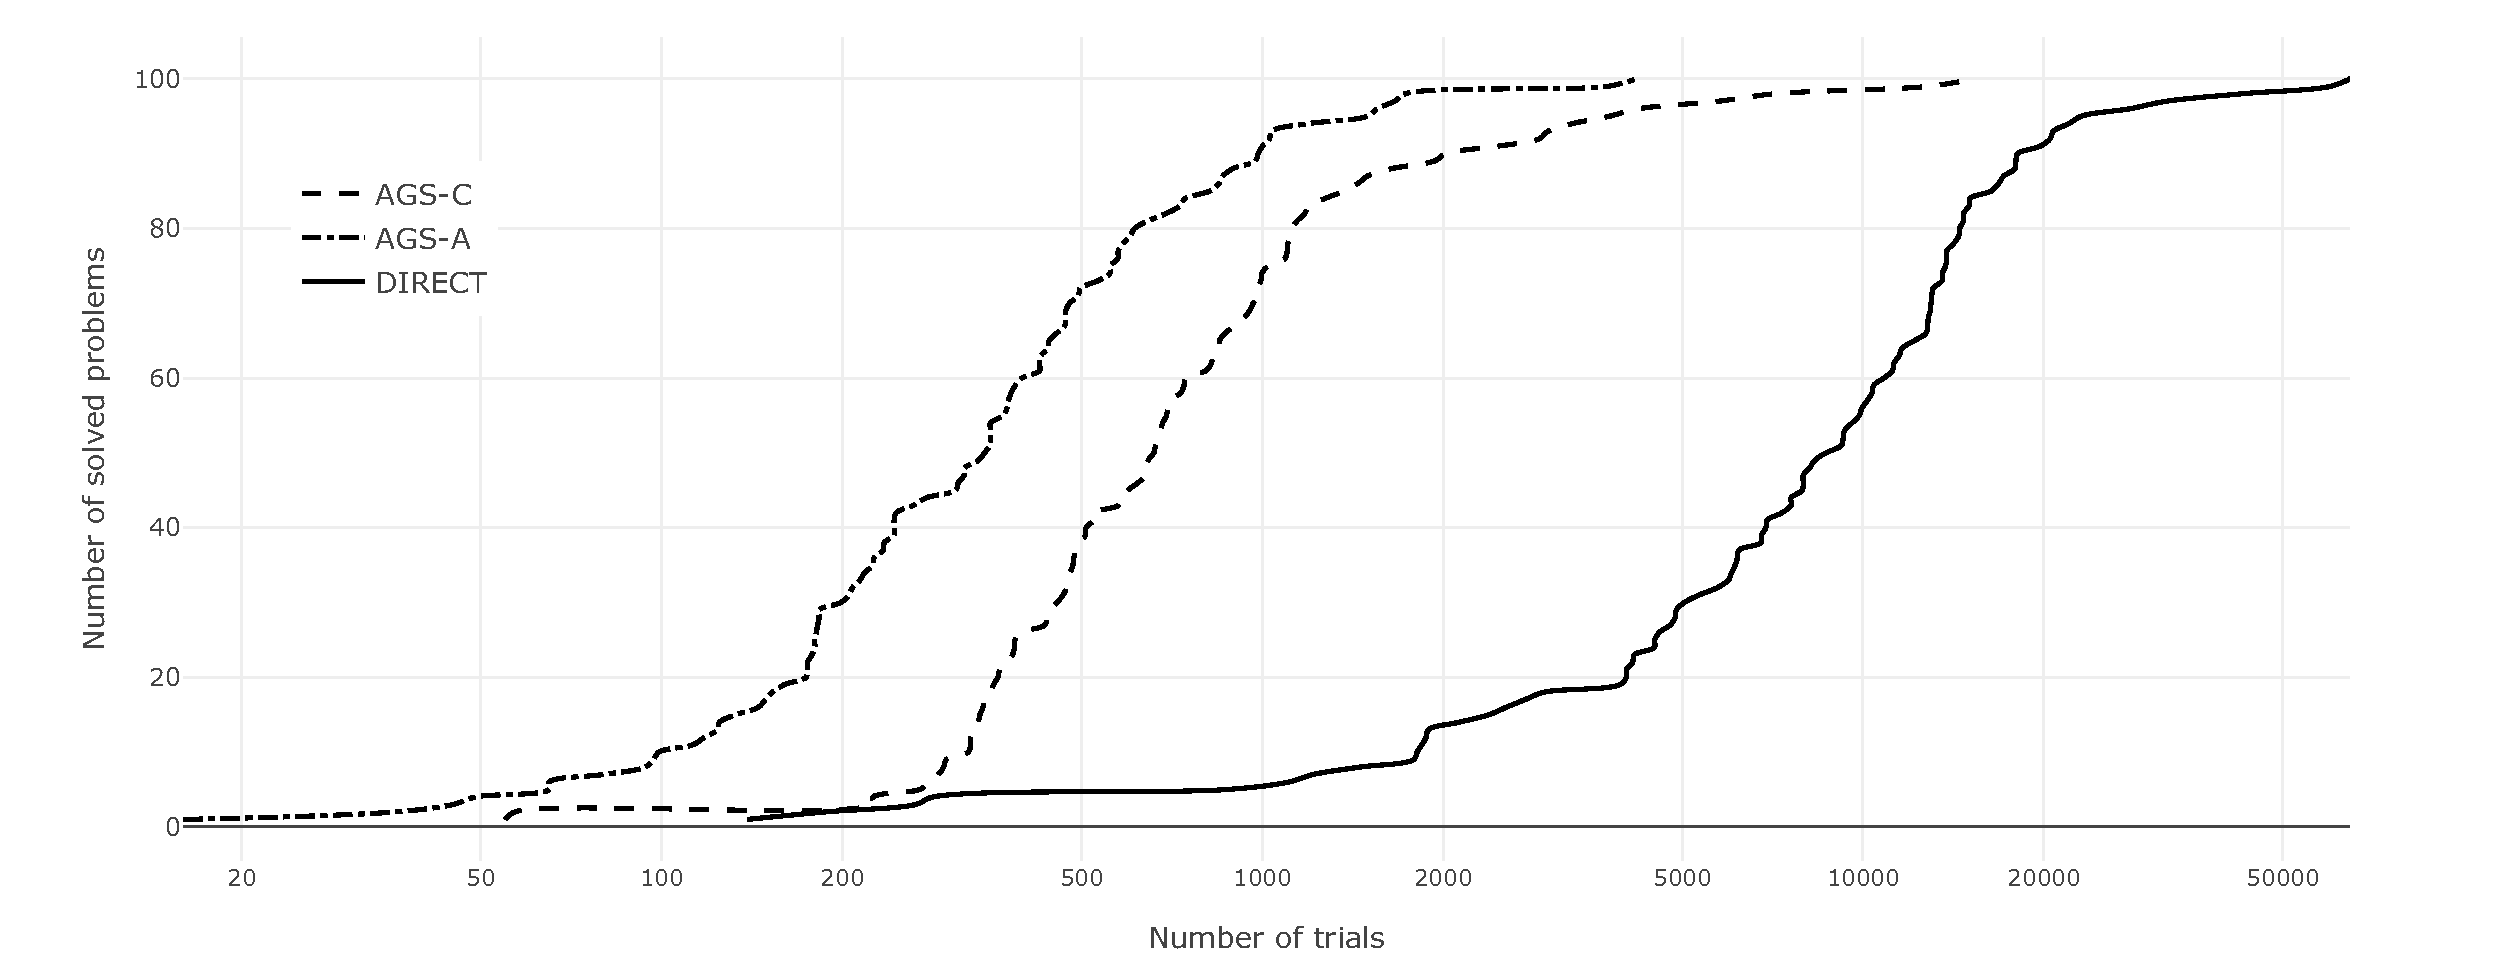
\includegraphics[width=1.0\linewidth]{figures/figure_5_11.pdf}
\caption{Operational characteristics of the nested optimization schemes and the method DIRECT.}
\label{fig:5_11}    
\end{figure}

As it follows from the presented examples and it is confirmed in other researches (see, for instance, \cite{5_GerGriGer, 5_GriIsrSergAIP, 5_GriIsrSergAMC}) the adaptive nested scheme improves significantly the results of optimization compared with its classical prototype. 

\subsection{Parallel adaptive scheme of nested optimization}
\label{subsec:5_4_3}
As well as the classical nested scheme, the adaptive one can be parallelized. The idea of parallelizing is similar to the approach applied in the parallel characteristical algorithms. Namely, when in a multiprocessor environment there are $p>1$ free processors, in the decision rule of the general stage for the choice of the subproblems for further solving one can take $p$ subproblems with the best characteristics. For more details, let us reformulate for the parallel case the general description of the sequential adaptive scheme modifying Steps G2-G4.

\paragraph{\textbf{General iteration of synchronous adaptive scheme}}
\begin{description} [\textbf{Step G1.}]
\item [\textbf{Step G1.}] {Juxtapose to each subproblem from the set $S$  a numerical value called characteristic of this problem.}
\item [\textbf{Step G2.}] {Choose $p$ subproblems with the greatest characteristics.}
\item [\textbf{Step G3.}]{Compute new trial points in the chosen subproblems and assign to each point one processor from the pool of free processors.}
\item [\textbf{Step G4.}]{Build in parallel the sub-trees of subtasks generated by these trial points in accordance with the nested scheme (\ref{eq:5_18})--(\ref{eq:5_21}) and add new subproblems of these sub-trees to the set $S$.}
\item [\textbf{Step G5.}]{If the termination  criterion is fulfilled in the root subproblem (\ref{eq:5_19}) stop the search and take as a result of optimization the least computed value of the objective function $\varphi(y)$ and its coordinates as the global minimizer. Otherwise, go to  \textbf{Step G1}.}
\end{description}

In this description, the computational parallel procedure is implicitly supposed to be synchronous since a new iteration G1-G5 can start after completion of  building all the sub-trees at Step G4 only.  Obviously, the times of building those can differ significantly. As a result, the processors completing computations wait until the slowest processor finishes and the new iteration of the general computational procedure can go on thereafter only. To avoid standing idle one can to use an asynchronous version of the parallel adaptive scheme presented below.

\paragraph{\textbf{General iteration of asynchronous adaptive scheme}}
\begin{description} [\textbf{Step G1.}]
\item [\textbf{Step G1.}] {If there are $1\leq\pi\leq p$ free processors go to \textbf{Step G2}. Otherwise, if there are no accessible processors, wait until $\pi,\:1\leq\pi\leq p$ processors have completed computations. After that add to the set $S$ new subproblems generated by processors having finished and go to the next \textbf{Step G2}.}
\item [\textbf{Step G2.}] {If the termination criterion is fulfilled in the root subproblem (\ref{eq:5_19}) stop the search and take as a result of optimization the least computed value of the objective function $\varphi(y)$ and its coordinates as the global minimizer. Otherwise, go to \textbf{Step G3}.}
\item [\textbf{Step G3.}]{Juxtapose to each subproblem from the set $S$ a numerical value called characteristic of this problem and choose $\pi$  subproblems with the greatest characteristic (the currently best subproblems).}
\item [\textbf{Step G4.}]{Compute new trial points in the chosen subproblems and assign to each point one processor from the pool of free processors.}
\item [\textbf{Step G5.}]{Begin solving subproblems generated by these trial points in accordance with the nested scheme  (\ref{eq:5_18})--(\ref{eq:5_21}) and go to \textbf{Step G1}.}
\end{description}

The description of general computational procedure for both the synchronous and asynchronous adaptive schemes is just a “skeleton” which requires many important details for a real implementation. For example, how to realize the stage of initialization, how to keep in memory the set of subproblems $S$, or how to organize the information exchange between processors?  It should be noted as well that in adaptive scheme the subproblems of a sub-tree do not required to be solved up to the end, i.e., up to fulfillment of termination criterion in univariate algorithm solving them as it is done in the classical nested scheme. In this situation the following question arises: how to stop the one-dimensional search during solving subproblems (\ref{eq:5_21})?  Moreover, the implementation of the adaptive scheme depends in many ways on the univariate methods use inside it. These and other peculiarities of possible implementation indicate a considerable variability of the adaptive scheme and require further investigations of increasing efficiency by means of new combinations of the general scheme with different univariate methods.

In conclusion some comparative results for the sequential and asynchronous versions of the adaptive scheme are presented. For the experiment the test class GKLS \cite{5_GavianoKvasovLeraSergeyev} was taken and test sets of functions for dimensions 7 and 8 were used. For univariate optimization inside the multidimensional search the information statistical method AGS was applied in all the cases. Computations were executed on a cluster consisting of 4 nodes with 4 processors Intel® Xeon® E7-8890 v4 and each processor contained 24 cores. Parallelization was realized on the base of MPI in the version Intel® MPI 2017. The interconnector Infiniband FDR was used for data exchange between processors.

Fig. ~\ref{fig:5_12} shows the speed-up in time of the asynchronous adaptive scheme as compared to the sequential one.
\begin{figure}[ht]
\centering
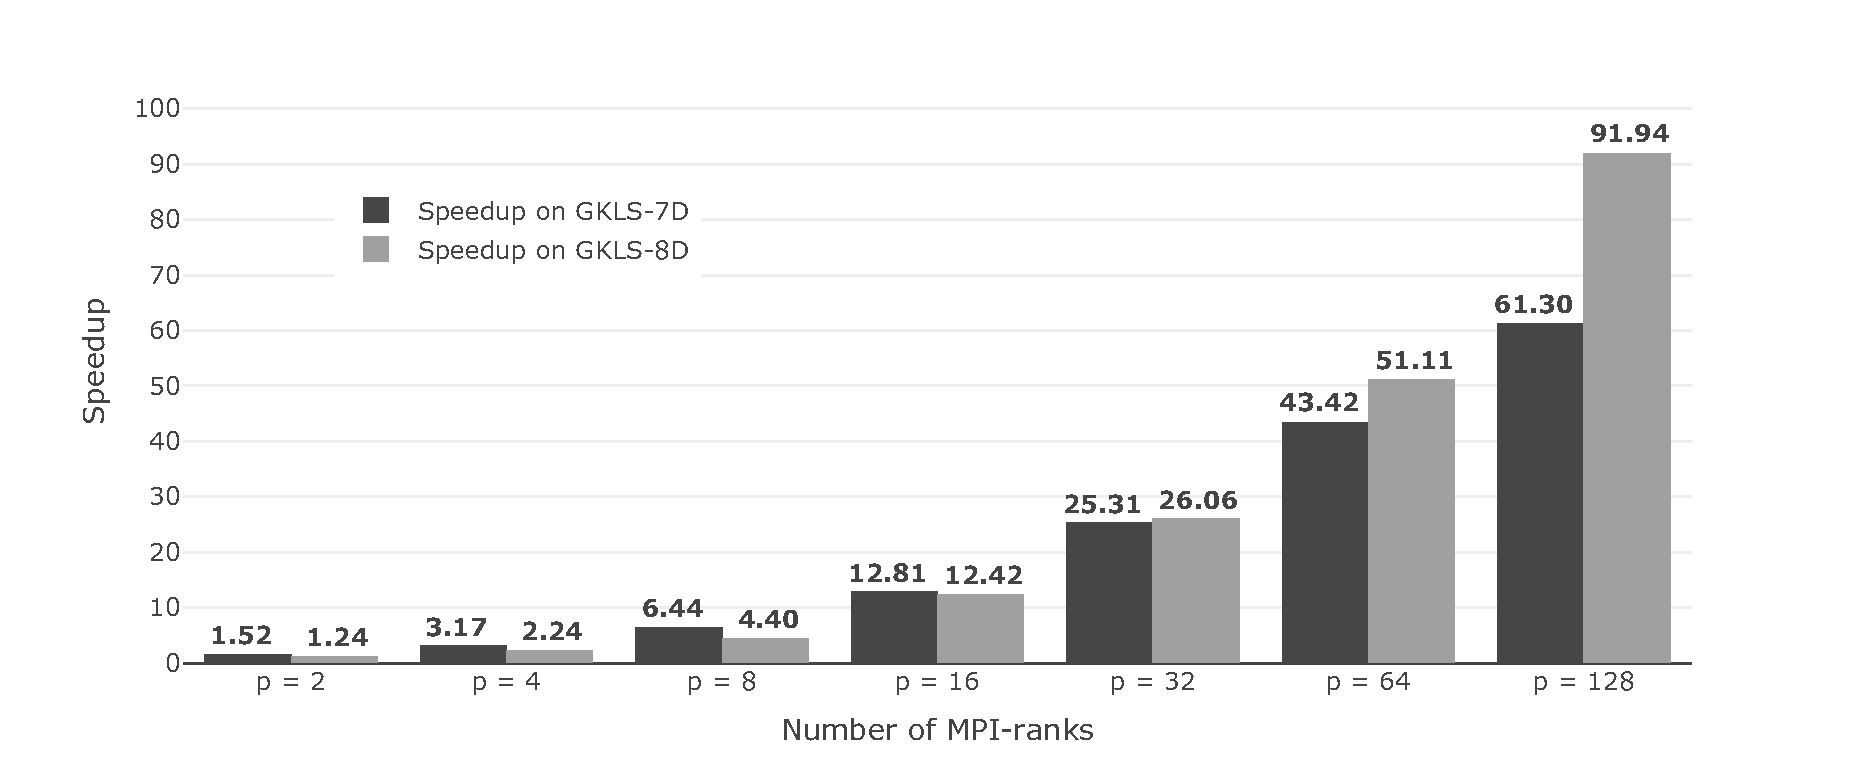
\includegraphics[width=1.05\linewidth]{figures/figure_5_12.pdf}
\caption{Speed-up of the asynchronous adaptive scheme.}
\label{fig:5_12}    
\end{figure}

Presented results demonstrate the substantial acceleration of the optimization process if to use the parallel adaptive scheme. It should be noted that if the parallelism is realized  with  few number of ranks then the efficiency of parallelizing is better for problems of the less dimension, however, the growth of number of MPI ranks leads to increasing the speed-up for  problems with more dimension (for 128 ranks speed-up in 8-dimensional problems is almost 1.5 times more than in 7-dimensional case).

\begin{thebibliography}{99.}
\bibitem{5_BarkGer2014} Barkalov, K.A., Gergel, V.P.: Multilevel scheme of dimensionality reduction for parallel global search algorithms.  OPT-i 2014 -- 1st International Conference on Engineering and Applied Sciences Optimization, Proceedings, 2111--2124 (2014)
\bibitem{5_BarkGerLeb} Barkalov, K., Gergel, V., Lebedev, I.: Solving global optimization problems on GPU cluster  AIP Conference Proceedings \textbf{1738}, 400006 (2016)
\bibitem{5_BarkLeb} Barkalov, K., Lebedev, I.: Local tuning in multilevel scheme of parallel global optimization.  AIP Conference Proceedings \textbf{1776}, 060006 (2016)
\bibitem{5_CarrHowe}	Carr, C.R., Howe, C.W.: Quantitative Decision Procedures in Management and Economic: Deterministic Theory and Applications. McGraw-Hill, New York (1964)
\bibitem{5_Evtushenko}	Evtushenko, Yu.G.: Numerical Optimization Techniques. Translation Series in Mathematics and Engineering. Optimization Software  Inc., Publication Division, New York (1985)
\bibitem{5_GavianoKvasovLeraSergeyev} Gaviano, M., Kvasov, D.E., Lera, D., Sergeyev, Y.D.: Algorithm 829: Software for generation of classes of test functions with known local and global minima for global optimization. ACM Trans. Math. Software \textbf{29}(4), 469–480 (2003)
\bibitem{5_GerGriIsr} Gergel, V.,  Grishagin, V., Israfilov, R.: Local tuning in nested scheme of global optimization, Procedia Computer Science \textbf{51}, 865--874 (2015) 
\bibitem{5_GerGriGer}	Gergel, V., Grishagin, V., Gergel, A.: Adaptive nested optimization scheme for multidimensional global search, J. Glob. Opt. \textbf{66}, 35–51 (2016).
\bibitem{5_GrishaginOperChar}  Grishagin,V.A.: Operation characteristics of some global search algorithms, Problems of Statistical Optimization \textbf{7},  198--206 (1978). In Russian
\bibitem{5_GriIsrAIP}	Grishagin, V.A., Israfilov, R.A.: Global search acceleration in the nested optimization scheme. AIP Conf. Proc. \textbf{1738}, 400010 (2016)
\bibitem{5_GriIsrSergAIP} Grishagin, V., Israfilov, R., Sergeyev, Y.: Comparative efficiency of dimensionality reduction schemes in global optimization. AIP Conf. Proc. \textbf{1776}, 060011 (2016)
\bibitem{5_GriIsrSergAMC}	Grishagin, V.,  Israfilov, R., Sergeyev, Y.: Convergence conditions and numerical comparison of global optimization methods based on dimensionality reduction schemes. Appl. Math.  Comput. (2017) doi:10.1016/j.amc.2017.06.036
\bibitem{5_GriIsrCEUR}Grishagin, V.A., Israfilov, R.A.: Multidimensional Constrained Global Optimization in Domains with Computable Boundaries. CEUR Workshop Proceedings \textbf{1513}, 75--84 (2015)
\bibitem{5_GrishaginSergeyevStrongin} Grishagin, V.A., Sergeyev, Y.D., Strongin, R.G.: Parallel characteristical algorithms for solving problems of global optimization. J. Global Optim. \textbf{10}(2), 185–206 (1997)
\bibitem{5_GrishaginStrongin_EnginCybernetics} Grishagin, V.A., Strongin, R.G.: Optimization of multiextremal functions subject to monotonically unimodal constraints. Engineering Cybernetics \textbf{22},  117--122 (1984)
\bibitem{5_Jones}Jones, D.R.: The DIRECT global optimization algorithm. In: C.A. Floudas, P.M. Pardalos
(eds.) Encyclopedia of Optimization, vol. 1, pp. 431–440. Kluwer Academic Publishers, Dordrecht (2001)
\bibitem{5_JonesPerttunenStuckman}Jones, D.R., Perttunen, C.D.,   Stuckman, B.E.: Lipschitzian optimization
without the Lipschitz constant, J. Optim. Theory Appl. 79,  157--181 (1993)
\bibitem{5_Kushner}	Kushner, H.J.: A new method of locating the maximum point of an arbitrary multipeak curve in the presence of noise. Transactions of ASME, Ser. D. Journal of Basic Engineering \textbf{86}, 97--106 (1964)
\bibitem{5_Locatelli} Locatelli, M.: Bayesian algorithms for one-dimensional global optimization. Journal of Global Optimization \textbf{1}, 57--76 (1997)
\bibitem{5_LucidiPiccioni} Lucidi, S., Piccioni, M.:  Random tunneling by means of acceptance-rejection sampling for global optimization. J. Optim. Theory Appl. \textbf{62}(2), 255--277 (1989)
\bibitem{5_Mockus1980} Mockus, J.: The simple Bayesian algorithm for the multidimensional global optimization. In: Archetti, F., and Cugiani, M. (Eds.) Numerical Techniques for Stochastic Systems. North-Holland, Amsterdam,
the Netherlands (1980)
\bibitem{5_Mockus1988}	Mockus, J.: Bayesian Approach to Global Optimization. Kluwer Academic Publishers, Dordrecht (1988)
\bibitem{5_MockusEddy_et_al} Mockus, J., Eddy, W., Mockus, A., Mockus, L., Reklaitis, G.: Bayesian Heuristic Approach
to Discrete and Global Optimization. Kluwer Academic Publishers, Dordrecht (1996)
\bibitem{5_Piyavskij}	Piyavskij, S.A.: An Algorithm for Finding the Absolute Extremum of a Function. USSR Comput. Math. Math. Phys. \textbf{12}(4), 57--67 (1972)
\bibitem{5_SergeyevLocTun} Sergeyev, Y.D.: An information global optimization algorithm with local tuning. SIAM J. Optim. \textbf{5}(4), 858–870 (1995)
\bibitem{5_Sergeyev1998} Sergeyev, Y.D.: Global one-dimensional optimization using smooth auxiliary functions. Math. Program. \textbf{81}(1), 127–146 (1998)
\bibitem{5_SergeyevGrishaginOMS} Sergeyev, Y.D., Grishagin, V.A.: Sequential and parallel algorithms for global optimization, Optim. Methods Softw. \textbf{3},  111--124 (1994)
\bibitem{5_SergGriJCAA}	Sergeyev, Y.D., Grishagin, V.A.: Parallel Asynchronous Global Search and the Nested Optimization Scheme. J. Comp. Analysis Appl. \textbf{3}, 123--145 (2001)
\bibitem{5_SergMukhKvasLera} Sergeyev, Y.D., Mukhametzhanov, M.S., Kvasov, D.E., Lera, D.: Derivative-free local tuning and local improvement techniques embedded in the univariate global optimization. J. Optim. Theory Appl. 171(1), 186--208 (2016)
\bibitem{5_ShiOlaf}   Shi, L., {\'O}lafsson, S.: Nested Partitions Method for Global Optimization. Operations Research \textbf{48}, 390--407 (2000)
\bibitem{5_Shubert} Shubert, B.O.: A sequential method seeking the global maximum of a function. SIAM J. Numer. Anal. \textbf{9}(3), 379–388 (1972)
\bibitem{5_StrMonRus}	Strongin, R.G.: Numerical Methods in Multiextremal Problems (Information-Statistical Algorithms). Nauka, Moscow (1978). In Russian
\bibitem{5_Str1973} Strongin, R.G.: On the convergence of an algorithm for finding a global extremum. Engineering Cybernetics 11, 549–555 (1973)
\bibitem{5_StrMarkin} Strongin, R.G., Markin, D.L.: Minimization of multiextremal functions with nonconvex constraints. Cybernetics 22, 486–493 (1986)
\bibitem{5_StrSergMon2000} Strongin, R.G., Sergeyev, Y.D.: Global Optimization with Non-Convex Constraints. Sequential and Parallel Algorithms. Kluwer Academic Publishers, Dordrecht (2000) 
\bibitem{5_SysoyevBarkGerLeb} Sysoyev, A., Barkalov, K., Gergel, V., Lebedev, I.: MPI implementation of dimension reduction multilevel scheme for parallel solving the global optimization problems  CEUR Workshop Proceedings \textbf{1482}, 61--68 (2015)
\bibitem{5_vanDam}	van Dam, E.R., Husslage, B., Hertog, D. One-dimensional Nested Maximin Designs. J. Glob. Opt. \textbf{46}, 287--306 (2010)
\bibitem{5_Zilinskas1975} $\check{Z}$ilinskas, A.: One-step Bayesian method for the search of the optimum of one-variable functions. Cybernetics 1, 139--144 (1975)
\bibitem{5_Zilinskas1981} $\check{Z}$ilinskas, A.: Two algorithms for one-dimensional multimodal minimization. Mat. Operationsforsch. Statist. \textbf{12}, Ser. Optimization, 53--63 (1981)
\bibitem{5_Zilinskas1985} $\check{Z}$ilinskas, A.: Axiomatic characterization of a global optimization algorithm and investigation of its search strategy. Operations Research Letters \textbf{4}, 35--39 (1985)
\end{thebibliography}

%\end{document}